%! Author = vyleg
%! Date = 23.11.2023

% Preamble

\usepackage[utf8]{inputenc}
\usepackage[T2A]{fontenc}
\usepackage[russian]{babel}


\documentclass{bmstu}
\bibliography{parts/lib}

\usepackage{listings}
\lstset{
    literate=
    {а}{{\selectfont\char224}}1
    {б}{{\selectfont\char225}}1
    {в}{{\selectfont\char226}}1
    {г}{{\selectfont\char227}}1
    {д}{{\selectfont\char228}}1
    {е}{{\selectfont\char229}}1
    {ё}{{\"e}}1
    {ж}{{\selectfont\char230}}1
    {з}{{\selectfont\char231}}1
    {и}{{\selectfont\char232}}1
    {й}{{\selectfont\char233}}1
    {к}{{\selectfont\char234}}1
    {л}{{\selectfont\char235}}1
    {м}{{\selectfont\char236}}1
    {н}{{\selectfont\char237}}1
    {о}{{\selectfont\char238}}1
    {п}{{\selectfont\char239}}1
    {р}{{\selectfont\char240}}1
    {с}{{\selectfont\char241}}1
    {т}{{\selectfont\char242}}1
    {у}{{\selectfont\char243}}1
    {ф}{{\selectfont\char244}}1
    {х}{{\selectfont\char245}}1
    {ц}{{\selectfont\char246}}1
    {ч}{{\selectfont\char247}}1
    {ш}{{\selectfont\char248}}1
    {щ}{{\selectfont\char249}}1
    {ъ}{{\selectfont\char250}}1
    {ы}{{\selectfont\char251}}1
    {ь}{{\selectfont\char252}}1
    {э}{{\selectfont\char253}}1
    {ю}{{\selectfont\char254}}1
    {я}{{\selectfont\char255}}1
    {А}{{\selectfont\char192}}1
    {Б}{{\selectfont\char193}}1
    {В}{{\selectfont\char194}}1
    {Г}{{\selectfont\char195}}1
    {Д}{{\selectfont\char196}}1
    {Е}{{\selectfont\char197}}1
    {Ё}{{\"E}}1
    {Ж}{{\selectfont\char198}}1
    {З}{{\selectfont\char199}}1
    {И}{{\selectfont\char200}}1
    {Й}{{\selectfont\char201}}1
    {К}{{\selectfont\char202}}1
    {Л}{{\selectfont\char203}}1
    {М}{{\selectfont\char204}}1
    {Н}{{\selectfont\char205}}1
    {О}{{\selectfont\char206}}1
    {П}{{\selectfont\char207}}1
    {Р}{{\selectfont\char208}}1
    {С}{{\selectfont\char209}}1
    {Т}{{\selectfont\char210}}1
    {У}{{\selectfont\char211}}1
    {Ф}{{\selectfont\char212}}1
    {Х}{{\selectfont\char213}}1
    {Ц}{{\selectfont\char214}}1
    {Ч}{{\selectfont\char215}}1
    {Ш}{{\selectfont\char216}}1
    {Щ}{{\selectfont\char217}}1
    {Ъ}{{\selectfont\char218}}1
    {Ы}{{\selectfont\char219}}1
    {Ь}{{\selectfont\char220}}1
    {Э}{{\selectfont\char221}}1
    {Ю}{{\selectfont\char222}}1
    {Я}{{\selectfont\char223}}1,
    % Добавляем параметры рамки
    frame=single,            % Одинарная рамка вокруг кода
    framesep=3pt,            % Отступ текста от рамки
    framexleftmargin=5pt,    % Отступ рамки слева
    framexrightmargin=5pt,   % Отступ рамки справа
    framextopmargin=5pt,     % Отступ рамки сверху
    framexbottommargin=5pt,  % Отступ рамки снизу
    backgroundcolor=\color{white}, % Фон листинга (можно заменить на светло-серый)
    rulecolor=\color{black}  % Цвет рамки
}

\usepackage[final]{pdfpages}
\pdfcompresslevel=9
\renewcommand\labelitemi{---} % Маркерные списки по госту

\begin{document}
%    
\includepdf[pages=-]{titul}
    \setcounter{page}{2}


\begin{essay}{}
    Ключевые слова:
    3Д--реконструкция,
    построение карты глубин,
    методы структурного освещения,
    определения глубины из размытия (Depth from defocus),
    стереосопоставления,
    структуры из движения (Structure from motion),
    комфортной генерации глубины (Comfortable Depth Generation).
%
%    Цель работы: классификация методов конвертации 2Д изображений в 3Д.
%
%    Данная научно--исследовательская работа включает
%    анализ предметной области,
%    описание основных подходов к решению задачи конвертации 2Д изображений в 3Д,
%    определение критериев сравнения,
%    и классификацию методов.
\end{essay}
    \def\contentsname{\hfill\centering СОДЕРЖАНИЕ\hfill}
    \makeatother

     % Добавление точек для глав в содержании
     \makeatletter
     \renewcommand*\l@chapter[2]{%
       \ifnum \c@tocdepth >\m@ne
         \vskip 1.0em \@plus\p@
         \setlength\@tempdima{1.5em}%
         \begingroup
           \parindent \z@ \rightskip \@pnumwidth
           \parfillskip -\@pnumwidth
           \leavevmode \bfseries
           \advance\leftskip\@tempdima
           \hskip -\leftskip
           #1\nobreak
           \leaders\hbox{$\m@th\mkern \@dotsep mu\box{.}\mkern \@dotsep mu$}\hfill
           \nobreak\hb@xt@\@pnumwidth{\hss #2}\par
         \endgroup
       \fi}
     \makeatother

     \tableofcontents
    \chapter*{ВВЕДЕНИЕ}
\addcontentsline{toc}{chapter}{ВВЕДЕНИЕ}

% TODO отчитать введение

Трехмерная реконструкция представляет собой процесс создания цифровых 3D-моделей объектов и сцен на основе двумерных изображений.
Это одно из активно развивающихся направлений на стыке компьютерного зрения, графики и машинного обучения.
Ключевым компонентом процесса является построение карты глубины — двумерной структуры данных, где каждый элемент соответствует расстоянию от камеры до объекта в реальном мире.
На основе подобных карт становится возможным восстановление объемной структуры сцены.

Технологии трехмерной реконструкции находят широкое применение в различных областях:
\begin{itemize}[wide=12.5mm, leftmargin=12.5mm]
    \item медицина~\cite{kt, med2, med3},
    \item культура и история~\cite{kult1, kult2},
    \item промышленное производство~\cite{prom1, prom2, prom3},
    \item индустрия развлечений~\cite{play1, play2, play3},
    \item системы компьютерного зрения~\cite{vis1, vis2, vis3}.
\end{itemize}

Работа с архивными фотографиями представляет особый интерес в контексте трехмерной реконструкции по следующим причинам:

\begin{enumerate}
    \item \textbf{Сохранение культурного наследия}: Архивные фотографии зачастую являются единственными свидетельствами существования утраченных культурных объектов, архитектурных сооружений и исторических ландшафтов. Их преобразование в трехмерный формат способствует более полному сохранению исторической памяти.
    
    \item \textbf{Научная и образовательная ценность}: Трехмерные реконструкции исторических объектов открывают новые возможности для исследований и образовательных проектов, делая историческое наследие более доступным и понятным для широкой аудитории.
    
    \item \textbf{Специфика исходных данных}: Архивные фотографии характеризуются различными видами деградации (выцветание, пятна, физические повреждения), неоднородным освещением и отсутствием дополнительной метаинформации, что требует разработки специализированных алгоритмов реконструкции.
\end{enumerate}

Разработанный в рамках данной работы гибридный метод восстановления глубины из монокулярных архивных изображений обладает следующими инновационными характеристиками:

\begin{enumerate}
    \item \textbf{Комбинирование подходов}: Предложенный метод объединяет преимущества нейросетевого подхода (MiDaS), обеспечивающего точное восстановление общей геометрии сцены, и классического метода Shape from Shading (SFS), сохраняющего детализацию и устойчивость к деградации.
    
    \item \textbf{Адаптивность к качеству изображений}: Метод динамически адаптирует стратегию восстановления в зависимости от степени деградации исходного материала, что особенно важно при работе с архивными фотографиями.
    
    \item \textbf{Устойчивость к дефектам}: Разработанное решение демонстрирует значительную устойчивость к типичным дефектам архивных фотографий, сохраняя приемлемую точность реконструкции даже при сильной деградации исходных изображений.
    
    \item \textbf{Отсутствие требований к обучающей выборке}: Метод не требует наличия обучающих данных с эталонной глубиной для архивных изображений, что делает его практически применимым в реальных сценариях работы с историческими коллекциями.
\end{enumerate}

\textbf{Цель работы}: Разработка и исследование гибридного метода восстановления трехмерной информации из архивных фотографий, устойчивого к различным типам деградации исходных изображений.

\textbf{Задачи исследования}:
\begin{enumerate}
    \item Провести анализ существующих методов восстановления глубины из монокулярных изображений и их применимости к архивным фотографиям.
    
    \item Разработать формальную модель гибридного метода, объединяющего нейросетевой подход (MiDaS) и классический метод Shape from Shading.
    
    \item Реализовать программный прототип предложенного метода с использованием современных технологий обработки изображений и машинного обучения.
    
    \item Провести экспериментальное исследование эффективности разработанного метода на изображениях с различной степенью деградации.
    
    \item Сформировать рекомендации по применению разработанного метода в зависимости от характеристик исходных архивных фотографий.
\end{enumerate}

Результаты исследования имеют прикладное значение для задач цифровой сохранности культурного наследия, виртуальных реконструкций исторических объектов и повышения доступности архивных материалов через их представление в современных цифровых форматах.

    \chapter{Аналитический раздел}

В области восстановления трехмерной формы объектов существует несколько подходов,
каждый из которых обладает своими особенностями и сферами применения.
Выбор метода зависит от требований к результату реконструкции, типа сцены, доступных данных и способов их получения.

В рамках данной работы будут рассмотрены методы восстановления глубины по единственному изображению:
\begin{itemize}
    \item структурного освещения,
    \item определения глубины из размытия (Depth from defocus)~\cite{dfd},
    \item комфортной генерации глубины (Comfortable Depth Generation),
    \item на основе нейронных сетей,
    \item восстановления глубины по закраске (Structure From Shadowing)~\cite{zaharov2011, zaharov2014}.
\end{itemize}

Задачами данного раздела являются:
\begin{itemize}
    \item обзор и сравнительный анализ существующих решений в области трехмерной реконструкции,
    \item формулировка цели работы,
    \item описание задач ВКР в виде функциональной модели.
\end{itemize}

\section{Метод структурного освещения}

В методе структурированного освещения используются различные типы световых паттернов,
которые проецируются на поверхность объекта.
Данные паттерны могут быть линейными, шахматными, градиентными и другими.
Пример паттерна представлен на изображении~\ref{pattern}.

\begin{figure}[H]
    \centering
    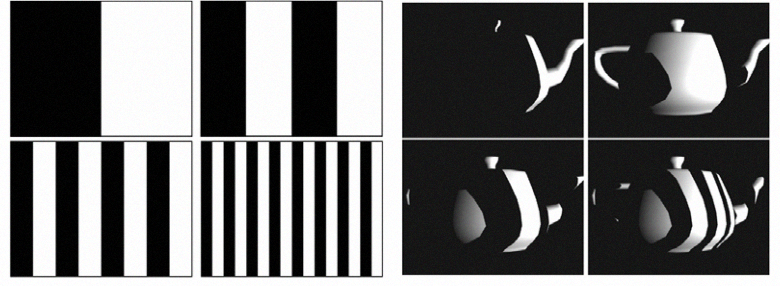
\includegraphics[scale=0.5]{img/pattern}
    \caption{Пример бинарных световых паттернов и освещенного с их помощью объекта~\cite{structLight}.}
    \label{pattern}
\end{figure}

Анализ искажений световых паттернов на поверхности объекта позволяет восстанавливать 3Д-геометрию объекта.
Основная задача метода заключается в выполнении триангуляции для определения расстояния от камеры до каждой точки поверхности.

На рисунке~\ref{metod1} приведена схема установки.

\begin{figure}[H]
    \centering
    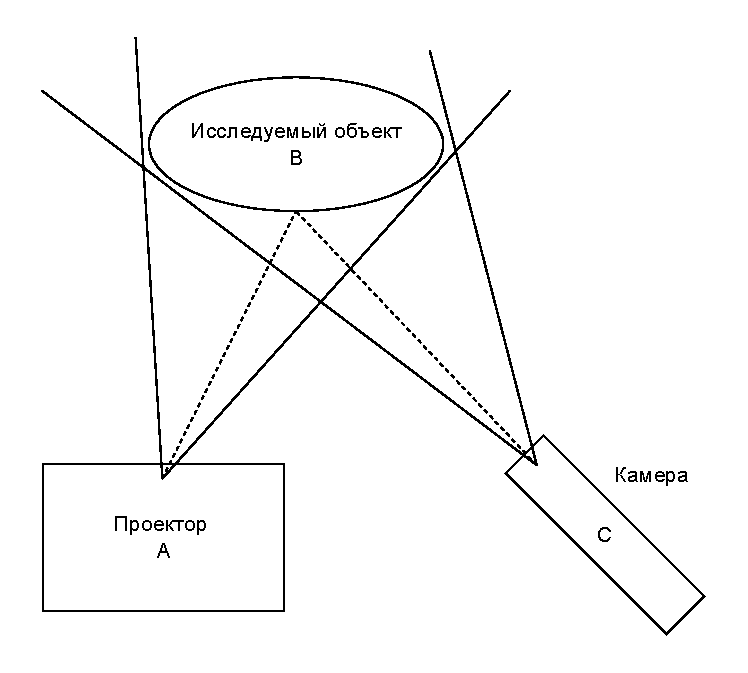
\includegraphics[scale=0.8]{img/metod1}
    \caption{Схема установки структурного освещения~\cite{structLight}.}
    \label{metod1}
\end{figure}

Создание карты глубин методом структурного освещения выполняется в несколько этапов~\cite{structLight}.

\begin{enumerate}[label=\arabic*.]
    \item \textbf{Калибровка камеры и проектора.} Определяются коэффициенты масштабирования ($\alpha_u$, $\alpha_v$), координаты оптического центра $(x_0, y_0)$ и фокусное расстояние $f$.
    \item \textbf{Проекция паттерна.} Проектор создает определенный световой шаблон (паттерн), который проецируется на исследуемую поверхность.
    \item \textbf{Фиксация изображения.} Камера фиксирует и регистрирует искажения паттерна на поверхности объекта.
    \item \textbf{Триангуляция.}
    \begin{enumerate}[label=\arabic{enumi}.\arabic*.]
        \item \textbf{ Вычисление углов.}

        Для вычисления расстояния от камеры до точки поверхности необходимо определить два угла треугольника \( \triangle ACB \):
        \begin{itemize}
            \item \( \angle CAB \) — угол между направлением от камеры \( C \) к проектору \( A \) и направлением от камеры \( C \) к точке на поверхности \( B \). Он вычисляется по формуле:
            \[
            \angle CAB = \arctan\left(\frac{x' - x_0}{f}\right),
            \]
            где \( x' \) — горизонтальная координата пикселя на изображении, \( x_0 \) — координата оптического центра камеры, а \( f \) — фокусное расстояние.

            \item \( \angle BCA \) — угол между направлением от точки \( B \) на поверхности к камере \( C \) и направлением от точки \( B \) к проектору \( A \). Он вычисляется по формуле:
            \[
            \angle BCA = \arctan\left(\frac{y' - y_0}{f}\right),
            \]
            где \( y' \) — вертикальная координата пикселя на изображении, \( y_0 \) — координата оптического центра камеры, а \( f \) — фокусное расстояние.
        \end{itemize}

        \item \textbf{Вычисление глубины $(BC)$ для каждой точки поверхности.}

        Используется триангуляция для определения расстояния \( BC \) от камеры до точки поверхности объекта:
        \begin{equation}
        BC = \frac{AC \cdot \sin(\angle CAB)}{\sin(\angle BCA)},
        \end{equation}
        где:
        \begin{itemize}
            \item \( AC \) — известное расстояние между камерой и проектором;
            \item \( \angle CAB \) и \( \angle BCA \) — углы треугольника \( \triangle ACB \), вычисляемые на предыдущем шаге.
        \end{itemize}

        \item \textbf{Преобразование координат изображения из 2Д- в 3Д-пространство.}

                Трёхмерные координаты точки поверхности \( (x, y, z) \) в системе камеры вычисляются по следующим формулам:
        \begin{equation}
        x = (x' - x_0) \cdot \frac{z}{\alpha_u}, \quad y = (y' - y_0) \cdot \frac{z}{\alpha_v}, \quad z = BC,
        \label{xyformula}
        \end{equation}
        где:
        \begin{itemize}
            \item \( x', y' \) — пиксельные координаты точки на изображении;
            \item \( \alpha_u, \alpha_v \) — коэффициенты масштабирования камеры по горизонтали и вертикали;
            \item \( x_0, y_0 \) — координаты оптического центра камеры.
        \end{itemize}
    \end{enumerate}
\end{enumerate}


Метод структурного освещения позволяет создавать точные и детализированные карты глубин,
что делает его незаменимым для решения задач,
в которых требуется высокая точность в определении расстояний до объектов.
Однако необходимым условием его использования является наличие специализированной лабораторной установки,
включающей камеру и проектор с точной калибровкой.
Такая установка требует стабильных условий и чувствительна к внешним факторам,
таким как освещенность или движение объекта.

Кроме того, метод ограничен размером и геометрией исследуемого объекта.
Структурированное освещение наиболее эффективно работает на объектах с относительно простой и ровной поверхностью.
Для сложных, сильно текстурированных или отражающих объектов,
качество получаемых данных значительно ухудшается из-за искажений паттернов,
что требует дополнительных техник для их компенсации.
Также метод неэффективен в условиях с ограниченным пространством,
где сложно разместить проектор и камеру под нужным углом.

\section{Метод определения глубины из размытия}

Метод оценки расстояний с использованием дефокусировки (Depth from Defocus, DFD) основан на анализе размытия изображения в точках, соответствующих границам объектов.
Предполагается, что перепад яркости на нерасфокусированном изображении границ объектов можно моделировать как ступенчатую функцию --- функцию Хевисайда~\cite{hewiside}.

Процесс оценки размытия выполняется в несколько этапов~\cite{dfd}.

\begin{enumerate}[label=\arabic*.]
\item \textbf{Выделение границ объектов.}
На изображении выделяются границы объектов, где наблюдаются значительные перепады яркости.
Эти границы служат ориентиром для дальнейшего анализа.
\item \textbf{Моделирование градиента яркости.}
Оценивается градиент яркости на выделенных границах объектов.
Этот шаг позволяет точно выявить изменения яркости, которые обусловлены дефокусировкой.
\item \textbf{Повторное размытие изображения.}
На изображение наносится дополнительное размытие, после чего вычисляется новый градиент яркости на границах объектов.
Это помогает уточнить степень дефокусировки, которая напрямую зависит от расстояния до объекта.
\item \textbf{Расчет параметра дефокусировки.}
На основе измерений градиента яркости и моделирования размытия вычисляется параметр дефокусировки, который используется для определения расстояния до объекта.
\end{enumerate}

Метод DFD показывает наилучшие результаты в случаях, когда есть возможность получить несколько снимков объекта с разными уровнями фокусировки.
Однако, результативность данного метода зависит от качества и точности модели размытия, а также от разрешения камеры.
В случае значительных искажений, например, при сильной дефокусировке или недостаточной контрастности на границах,
результаты менее точные.
Кроме того, для получения корректных результатов требуется тщательная настройка параметров камеры,
таких как диафрагма и фокусное расстояние.

\section{Метод комфортной генерации глубины}

Метод комфортной генерации глубины представляет собой подход,
который использует информацию о цветовых характеристиках блоков изображения для вычисления расстояния до объекта.

Процесс заключается в разбиении изображения на блоки, анализе их цветовых характеристик и применении минимальных остовных деревьев~\cite{minderev} для вычисления глубины.

Выделяют несколько основных этапов метода комфортной генерации глубины~\cite{comf}.

\begin{enumerate}[label=\arabic*.]
\item \textbf{Разбиение изображения на блоки.}
Изображение делится на блоки размером 4x4 пикселя, что позволяет упростить задачу обработки изображения и снизить вычислительную сложность.

\item \textbf{Вычисление среднего цвета для каждого блока.}
Для каждого блока вычисляется среднее значение цвета (mean(a)),
что представляет собой характеристику блока, на основе которой будет строиться граф для дальнейшей обработки.

\item \textbf{Построение графа.}
Изображение представляется как неориентированный граф \(G(V, E)\), где:
\begin{itemize}
    \item \(V\) — вершины графа, которые соответствуют блокам изображения;
    \item \(E\) — ребра графа с весами, которые рассчитываются как абсолютное различие средних значений цвета между соседними блоками, то есть \(|\text{mean(a)} - \text{mean(b)}|\).
\end{itemize}

\item \textbf{Построение минимального остовного дерева.}
На основе построенного графа применяется алгоритм Прима~\cite{prima} для нахождения минимального остовного дерева.
Этот шаг помогает упорядочить блоки по их взаимному сходству и устанавливает структуру для дальнейшего анализа.

\item \textbf{Разрезание дерева.}
После построения минимального остовного дерева выполняется его разрезание по ребрам с большими весами, что помогает выделить сегменты изображения, которые могут быть интерпретированы как части с различной глубиной.

\item \textbf{Выбор базового градиента глубины.}
Из анализа прямых линий на изображении выбирается один из базовых градиентов глубины.
Для этого используются параметры \(Wrl\) и \(Wud\), которые характеризуют градиент в двух направлениях (горизонтальном и вертикальном).
При этом выполняется условие \(|Wrl| + |Wud| = 1\).

\item \textbf{Вычисление глубины сегмента.}
Для каждого сегмента изображения глубина вычисляется как среднее значение глубины всех пикселей в сегменте.

\end{enumerate}

На рисунке~\ref{comf} приведен пример обработки одного блока изображения.

\begin{figure}[H]
    \centering
    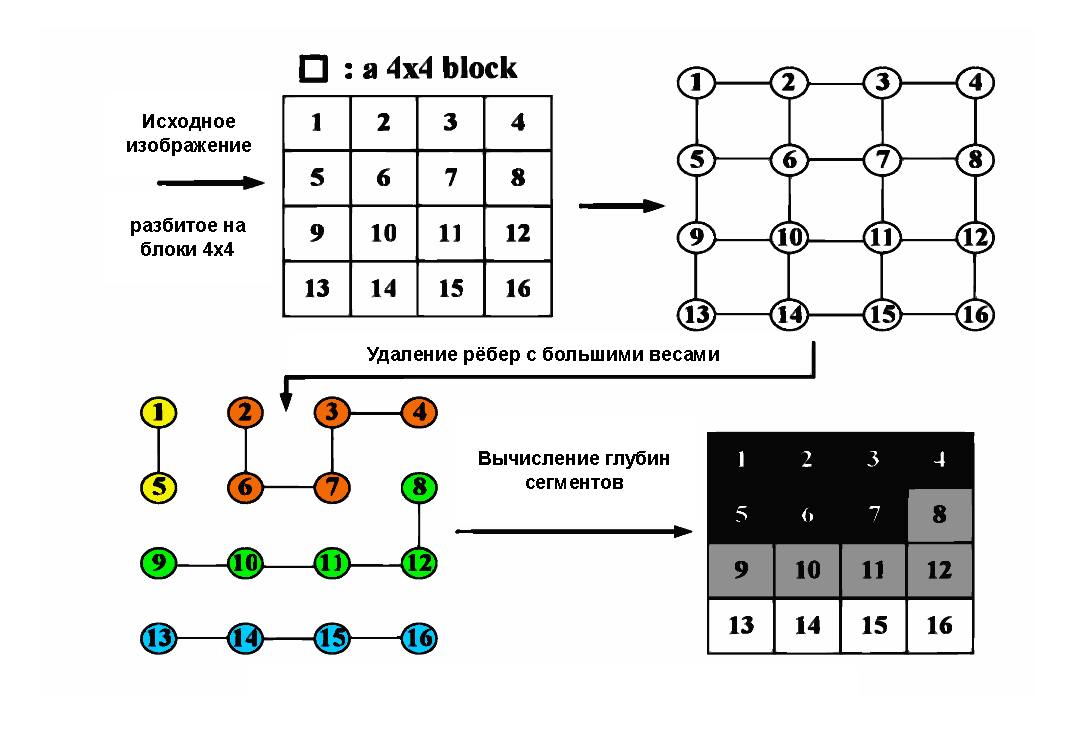
\includegraphics[scale=0.9]{img/comf}
    \caption{Обработка блока изображения~\cite{comf}.}
    \label{comf}
\end{figure}

Метод комфортной генерации глубины предполагает разбиение изображения на независимые части,
что позволяет обрабатывать данные параллельно.
Этот подход отличается универсальностью применения, поскольку может обрабатывать как локальные, так и глобальные сцены, не требуя при этом дополнительной информации или специального подхода к сбору данных.

Однако, метод Comfortable Depth Generation имеет некоторые ограничения,
связанные с качеством исходных изображений.
Низкое качество или низкая контрастность изображения снижает точность получаемой глубины.
Кроме того, фиксированный размер блоков (4x4 пикселя) ограничивает точность при обработке изображений с детализированными структурами,
требующими разделение на более мелкие части.
В случае с изображениями, содержащими гладкие или однотонные текстуры,
блоки имеют схожие цветовые характеристики,
что затрудняет выделение различных глубинных уровней.

\section{Метод восстановления глубины на основе нейронных сетей}

Методы восстановления глубины на основе нейронных сетей используют глубокое обучение для
выявления сложных статистических закономерностей между визуальными признаками 2D-изображения и соответствующими значениями глубины~\cite{shestopalov2024, istomin2024}.

Алгоритмы монокулярной оценки глубины можно разделить на несколько категорий в зависимости от их архитектуры
и подходов~\cite{istomin2024}.
Первая категория --- это предсказание глубины на основе свёрточных нейронных сетей (CNN)~\cite{istomin2024, istomin10}.
Свёрточные нейронные сети применяются для прямого предсказания карты глубин из изображения.
Обычно этот процесс заключается в обучении сети на наборах данных, содержащих пары изображений и соответствующих им карт
глубин, что позволяет модели эффективно улавливать глубинные характеристики сцены.

Второй тип архитектур --- это кодировщик-декодировщик,
в которых кодировщик отвечает за извлечение признаков из изображения, а декодировщик использует эти признаки для восстановления карты
глубин~\cite{istomin2024, istomin12}.
Такая структура позволяет более эффективно моделировать сложные зависимости в изображениях, что
повышает точность результата~\cite{istomin2024}.

Одним из представителей нейросетевых методов является модель MiDaS,
предназначенная для оценки глубины на основе одиночных изображений, которая характеризуется гибридной архитектурой,
объединяющей элементы кодера-декодера в рамках свёрточной нейронной сети~\cite{istomin2024, istomin12}.

MiDaS обучен на комбинированных наборах данных, что обеспечивает его универсальность для разных типов сцен
и устойчивость к шумам и артефактам.
Кроме того, важным преимуществом является отсутствие необходимости в знании точных параметров камеры и какой-либо дополнительной информации.
Однако, как и метод Comfortable Depth Generation, нейросетевые подходы ориентированы на восстановление общей структуры глубины, упуская детали поверхностей.

\section{Метод восстановления глубины по закраске изображения}

Метод Shape from Shading (SFS) --- это подход к восстановлению трехмерной формы объекта на основе анализа распределения интенсивности света и теней на двумерном изображении.
Этот метод базируется на физических принципах отражения света от поверхностей объектов.

Восстановление формы по закраске производится в несколько этапов~\cite{stanowski2024stability}.

\begin{enumerate}[label=\arabic*.]
\item \textbf{Определение модели освещения.}
Для анализа используется модель отражения, описывающая взаимосвязь между интенсивностью пикселя, нормалью к поверхности и направлением падающего света. Чаще всего применяется ламбертовская модель освещения:
\begin{equation}
I(x,y) = \rho(x,y) \cdot L \cdot N(x,y),
\end{equation}
где $I(x,y)$ --- интенсивность пикселя, $\rho(x,y)$ --- альбедо поверхности, $L$ --- направление источника света, $N(x,y)$ --- нормаль к поверхности.

\item \textbf{Разделение альбедо и затенения.}
Анализируется изменение яркости изображения для отделения свойств материала (альбедо) от эффектов затенения, вызванных геометрией поверхности.
Альбедо характеризует собственный цвет и отражательную способность материала.

\item \textbf{Вычисление нормалей поверхности.}
На основе интенсивности пикселей и модели освещения вычисляются нормали к поверхности в каждой точке.
Для каждого пикселя определяется вектор нормали $N(x,y)$, перпендикулярный к касательной плоскости поверхности.

\item \textbf{Интеграция нормалей.}
Для получения карты глубин выполняется интеграция поля нормалей.
Этот процесс можно представить как решение следующего уравнения:
\begin{equation}
\nabla Z(x,y) = f(N(x,y)),
\end{equation}
где $Z(x,y)$ --- искомая карта глубины, а $f$ --- функция, преобразующая нормали в градиент глубины.

\item \textbf{Применение регуляризации.}
Для преодоления неоднозначности решения и устранения шумов используются методы регуляризации, которые вводят дополнительные ограничения на гладкость поверхности.
\end{enumerate}

Метод SFS обладает рядом преимуществ, ключевым из которых является возможность восстановления 3D-формы объекта по одиночному изображению.
Это делает его применимым для работы с историческими фотографиями, когда невозможно получить несколько ракурсов объекта~\cite{xie2025photometric}.

Однако метод имеет существенные ограничения.
Во-первых, он требует точного знания параметров освещения, которые часто недоступны для архивных фотографий.
Во-вторых, базовая модель предполагает однородность материала поверхности, что редко встречается в реальных сценах.
В-третьих, метод дает неоднозначные результаты, поскольку различные 3D-формы могут создавать схожие паттерны затенения~\cite{zhang2025review}.



    \section{Классификация методов восстановления глубины}

На основе проведенного анализа предметной области были определены несколько ключевых критериев сопоставления рассмотренных методов.

\begin{enumerate}[label=\arabic*.]
    \item \textbf{Способ получения данных} --- активный или пассивный подход к сбору информации.

    Предложенный критерий учитывает подход к сбору исходных данных.
    Активные методы, такие как лазерное сканирование, требуют использования специализированного оборудования, что
    предполагает проведение исследований в лабораторных условиях.
    Пассивные методы, напротив, работают с доступными изображениями.
    Применение данного критерия позволяет своевременно
    оценить необходимые условия получения исходных изображений.

    \item \textbf{Дополнительная информация} --- данные о положении камер, временных метках и других параметрах.

    Необходимость в дополнительной информации ограничивает область применения метода и
    может предполагать наличие дополнительных компетенций для их использования, например, при настройке параметров камеры.

    \item \textbf{Результат} --- итоговый объект реконструкции (карта глубин, информация о структуре объекта).

    Базовым результатом является карта глубин, однако некоторые методы предоставляют дополнительную информацию:
    форма объекта, нормали к поверхностям.
    Эти дополнительные данные могут быть критически важны для полноценной трёхмерной реконструкции сцены.

    \item \textbf{Масштаб сцены} --- локальная или глобальная реконструкция.

    Масштаб сцены определяет применимость метода к задачам разного уровня: от реконструкции небольших объектов до глобальных ландшафтов.

    \item \textbf{Уровень автоматизации} --- степень автоматизированности процесса реконструкции: от ручных до автоматических методов.

    Уровень автоматизации влияет на затраты времени и ресурсов.
    Автоматизированные методы предпочтительны для задач, требующих быстрой обработки больших объемов данных,
    тогда как ручные обеспечивают больше контроля в специфических сценариях.
\end{enumerate}

Данные критерии позволяют выбрать наиболее подходящий метод восстановления глубины в зависимости от поставленной задачи,
доступных возможностей и особенностей предметной области.

В таблице~\ref{tab:methods_comparison} приведена классификация методов восстановления глубины.
\begin{table}[H]
    \centering
    \begin{tabular}{|p{2.4cm}|p{2.2cm}|p{2.6cm}|p{2.2cm}|p{2.3cm}|p{3.1cm}|}
        \hline
        Метод & Способ \newline получения данных & Доп. \newline информация & Результат & Масштаб сцены & Уровень \newline автоматизации \\
\noalign{\hrule height 2pt}
        Метод структурного освещения & Активный & Проекция шаблона & Карта глубин, форма объекта  & Локальные & Ручные \\
        \hline
        DFD & Активный или \newline пассивный & Параметры настройки камеры & Карта глубин & Локальные & Автономные \\
        \hline
        Shape from Shading (SFS) & Пассивный & Параметры освещения & Карта глубин, нормали поверхности & Локальные & Полу-автономные \\
        \hline
        Comfortable depth generation & Пассивный & - & Карта глубин & Локальные или \newline глобальные & Автономные \\
        \hline
        MiDaS & Пассивный & - & Карта глубин & Локальные или \newline глобальные & Автономные \\
        \hline
    \end{tabular}
    \caption{Классификация методов восстановления глубины из монокулярных изображений}
    \label{tab:methods_comparison}
\end{table}

\section{Выбор метода восстановления глубины архивных фотографий}

При выборе метода для восстановления глубины из старинных фотографий необходимо учитывать их специфические особенности и ограничения.

\begin{enumerate}
    \item \textbf{Ограниченность исходных данных}. Для архивных фотографий доступны только одиночные изображения, отсутствует возможность получения стереопар или последовательностей с разных ракурсов.

    \item \textbf{Отсутствие метаданных}. Архивные фотографии не содержат информации о параметрах съемки, калибровке камеры или условиях освещения.

    \item \textbf{Качество изображений}. Старинные фотографии часто имеют низкое качество, шумы, артефакты, выцветание и повреждения, что затрудняет автоматическую обработку.
\end{enumerate}

Исходя из представленной классификации, рассмотрим применимость каждого метода.

\textbf{Метод структурированного освещения} и \textbf{DFD} требуют активного вмешательства при съемке или специальных параметров камеры, что делает их неприменимыми для архивных фотографий.

\textbf{Shape from Shading} работает с моноизображениями и может восстанавливать форму объектов на основе анализа теней и освещения.
Однако метод имеет существенные ограничения: необходимость в параметрах освещения, которые невозможно достоверно определить для архивных фотографий, и применимость преимущественно к локальным сценам с четко выраженными текстурами и тенями.
Тем не менее, возможна разработка адаптированного алгоритма, в котором параметры освещения оцениваются на основе самого изображения, а область применения включает более сложные сцены за счет сегментации изображения.

\textbf{Comfortable depth generation} представляется подходящим методом, поскольку он работает с моноизображениями и не требует дополнительной информации.
Однако, для архивных фотографий с их специфическими искажениями нейросетевые подходы предположительно демонстрируют более высокую устойчивость и точность.

\textbf{Нейросетевые методы}, в частности MiDaS, представляются наиболее подходящим решением, поскольку они:
\begin{itemize}
    \item работают с одиночными изображениями,
    \item не требуют дополнительной информации о сцене или камере,
    \item обеспечивают полностью автоматическую обработку,
    \item демонстрируют высокую точность на разнообразных сценах благодаря обучению на больших наборах данных,
    \item эффективно работают как с локальными, так и с глобальными сценами, хотя качество детализации при работе с глобальными сценами снижается.
\end{itemize}

Таким образом, для повышения качества результатов разумно использовать гибридный подход:
комбинировать \textbf{нейросетевой метод} (MiDaS) для получения базовой карты глубин с элементами \textbf{Shape from Shading} для улучшения детализации в областях с выраженной текстурой и тенями.

При этом необходимо учитывать особенности архивных фотографий, реализовав предварительную обработку для устранения артефактов и повреждений, снижения шума, повышения контраста, восстановления насыщенности и других параметров изображения.

\section{Цель и постановка задачи}

Целью данной работы является разработка метода восстановления трехмерной глубины из архивных фотографий путем создания гибридного алгоритма, объединяющего преимущества нейросетевого метода и Shape from Shading, с учетом специфических особенностей исторических изображений.

Формально задачу восстановления карты глубины из архивной фотографии можно представить как функциональную модель:

\begin{equation}
D = F(I, P),
\end{equation}

где:
\begin{itemize}
    \item $D : \mathbb{R}^2 \to \mathbb{R}$ --- искомая карта глубин, сопоставляющая каждой точке $(x, y)$ изображения значение глубины;
    \item $I : \mathbb{R}^2 \to \mathbb{R}^3$ --- исходное изображение, представленное как функция, сопоставляющая каждой точке $(x, y)$ цвет в формате RGB;
    \item $P$ --- набор параметров алгоритма;
    \item $F$ --- оператор преобразования, реализующий гибридный метод.
\end{itemize}

Оператор $F$ представляет собой композицию следующих функций:

\begin{equation}
F = F_{\text{post}} \circ F_{\text{hybrid}} \circ F_{\text{pre}},
\end{equation}

где:
\begin{itemize}
    \item $F_{\text{pre}} : \mathbb{R}^2 \times \mathbb{R}^3 \to \mathbb{R}^2 \times \mathbb{R}^3$ --- функция предобработки, выполняющая шумоподавление, коррекцию яркости и контраста;
    \item $F_{\text{hybrid}} : \mathbb{R}^2 \times \mathbb{R}^3 \to \mathbb{R}^2 \times \mathbb{R}$ --- гибридная функция, объединяющая методы MiDaS и SFS;
    \item $F_{\text{post}} : \mathbb{R}^2 \times \mathbb{R} \to \mathbb{R}^2 \times \mathbb{R}$ --- функция постобработки, выполняющая сглаживание и нормализацию карты глубин.
\end{itemize}

Гибридная функция $F_{\text{hybrid}}$ определяется как:

\begin{equation} F_{\text{hybrid}}(I) = \alpha_{map} \cdot F_{\text{MiDaS}}(I) + (1 - \alpha_{map}) \cdot F_{\text{SFS}}(I), \end{equation}

где: \begin{itemize} \item $F_{\text{MiDaS}}$ --- базовая карта глубин, полученная методом MiDaS;
\item $F_{\text{SFS}}$ --- карта деталей, полученная методом Shape from Shading;
\item $w_{detail}(x,y)$ --- карта весов деталей, определяющая их значимость;
\item $\alpha_{map}(x,y)$ --- адаптивный весовой коэффициент, уменьшающийся в областях с высокой детализацией.
\end{itemize}

\section*{Вывод}

В аналитической части работы проведен обзор существующих способов восстановления глубины по единственной фотографии, а именно
методы структурного освещения, Depth from defocus, Shape from Shading, Comfortable Depth Generation и нейросетевые методы, такие как MiDaS.

Рассмотренные подходы классифицированы по ключевым критериям:
способу получения данных, необходимости в дополнительной информации, результатам реконструкции, масштабу сцены и уровню автоматизации.

Проведенный анализ позволяет сделать вывод, что оптимальным решением для восстановления глубины из архивных фотографий является гибридный метод,
объединяющий преимущества нейросетевого подхода (MiDaS) и классического метода Shape from Shading.
Такой подход обеспечивает как общую точность восстановления геометрии сцены,
так и детализацию отдельных элементов, сохраняя при этом устойчивость к дефектам, характерным для исторических изображений.

Представленное формализованное описание задач в виде функциональной модели, включающей блоки предобработки,
гибридного восстановления и постобработки, формируют теоретическую основу для разработки практического решения в следующих разделах работы.


    \chapter{Конструкторский раздел}

В данном разделе формализована структура разработанного метода,
описана алгоритмическая основа функциональных блоков и их взаимодействия в рамках единой системы.

Структура решения представлена в виде IDEF0--диаграммы и подробных схем для каждого этапа обработки:
предварительной подготовки изображений, сегментации, оценки освещения, разделения альбедо и затенения,
расчета нормалей к поверхности и итогового восстановления трехмерной информации.

\section{IDEF-0 диаграммы}

На рисунке~\ref{idef0-a0} представлена диаграмма IDEF0 уровня A0 разработанного метода.

% TODO убрать из А0 управление метрики качества + добавить параметры алгоритмов к управлению на А1

\begin{figure}[H]
    \centering
    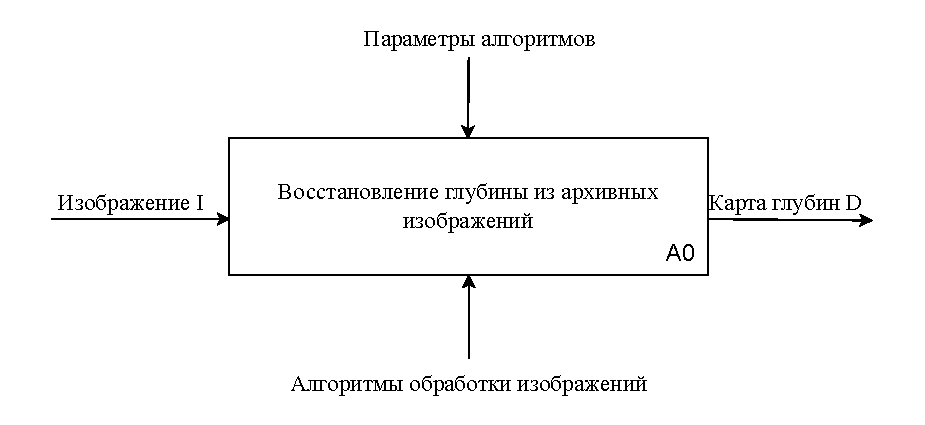
\includegraphics[scale=0.8]{img/IDEFA0}
    \caption{IDEF0-диаграмма уровня A0}
    \label{idef0-a0}
\end{figure}

Диаграмма нулевого уровня представляет всю систему как единый блок с указанием входов, выходов, управления и механизмов.
Входными данными системы являются архивные фотографии, выходными --- восстановленная карта глубин.

На рисунке~\ref{idef0-a1} показана декомпозиция функционального блока A0, детализирующая основные процессы обработки изображений.

\begin{figure}[H]
    \centering
    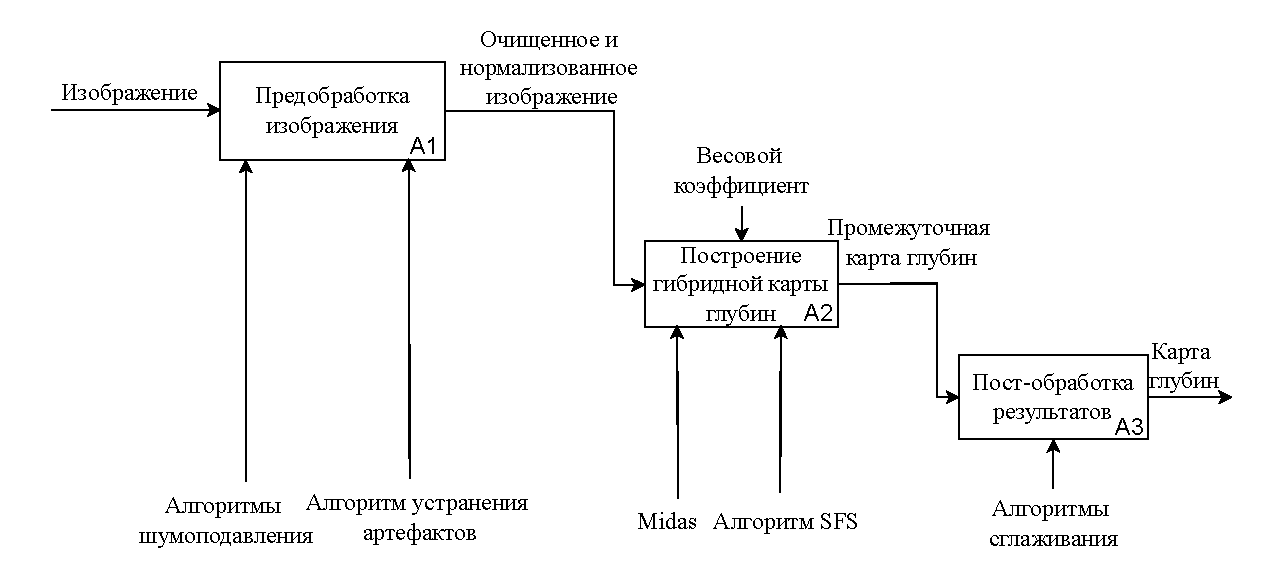
\includegraphics[scale=0.8]{img/IDEFA1}
    \caption{IDEF0-диаграмма уровня A1}
    \label{idef0-a1}
\end{figure}

Диаграмма уровня A1 визуализирует три основных функциональных блока системы: предобработка, гибридное восстановление и постобработка.
Отражены их взаимосвязи, потоки данных между блоками, управляющие воздействия и используемые механизмы.

%Рисунок~\ref{idef0-a2} демонстрирует декомпозицию второго блока диаграммы A1 --- процесса гибридного восстановления.
%
%\begin{figure}[H]
%    \centering
%    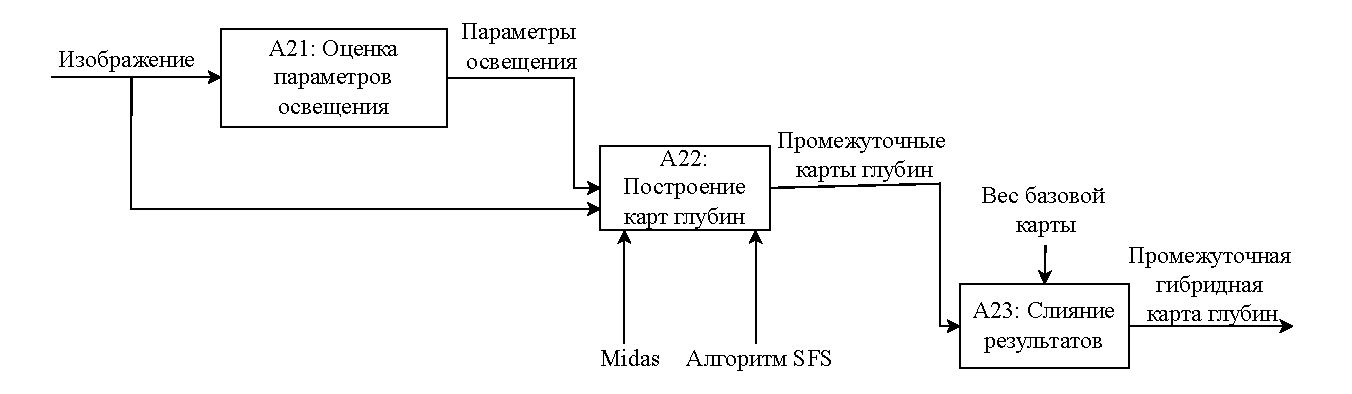
\includegraphics[scale=0.8]{img/IDEFA2}
%    \caption{IDEF0-диаграмма уровня A2}
%    \label{idef0-a2}
%\end{figure}
%
%На диаграмме уровня A2 детализирован процесс гибридного восстановления, включающий сегментацию изображения,
%оценку освещения, применение нейросетевого метода и метода Shape from Shading, а также интеграцию результатов.
%На этом этапе формируются ключевые промежуточные представления для каждого из используемых методов.

\section{Схемы алгоритмов}

На рисунке~\ref{preobr} представлена схема предварительной обработки входного изображения, включающая методы шумоподавления, нормализации освещения и коррекции артефактов, характерных для архивных фотографий.

\begin{figure}[H]
    \centering
    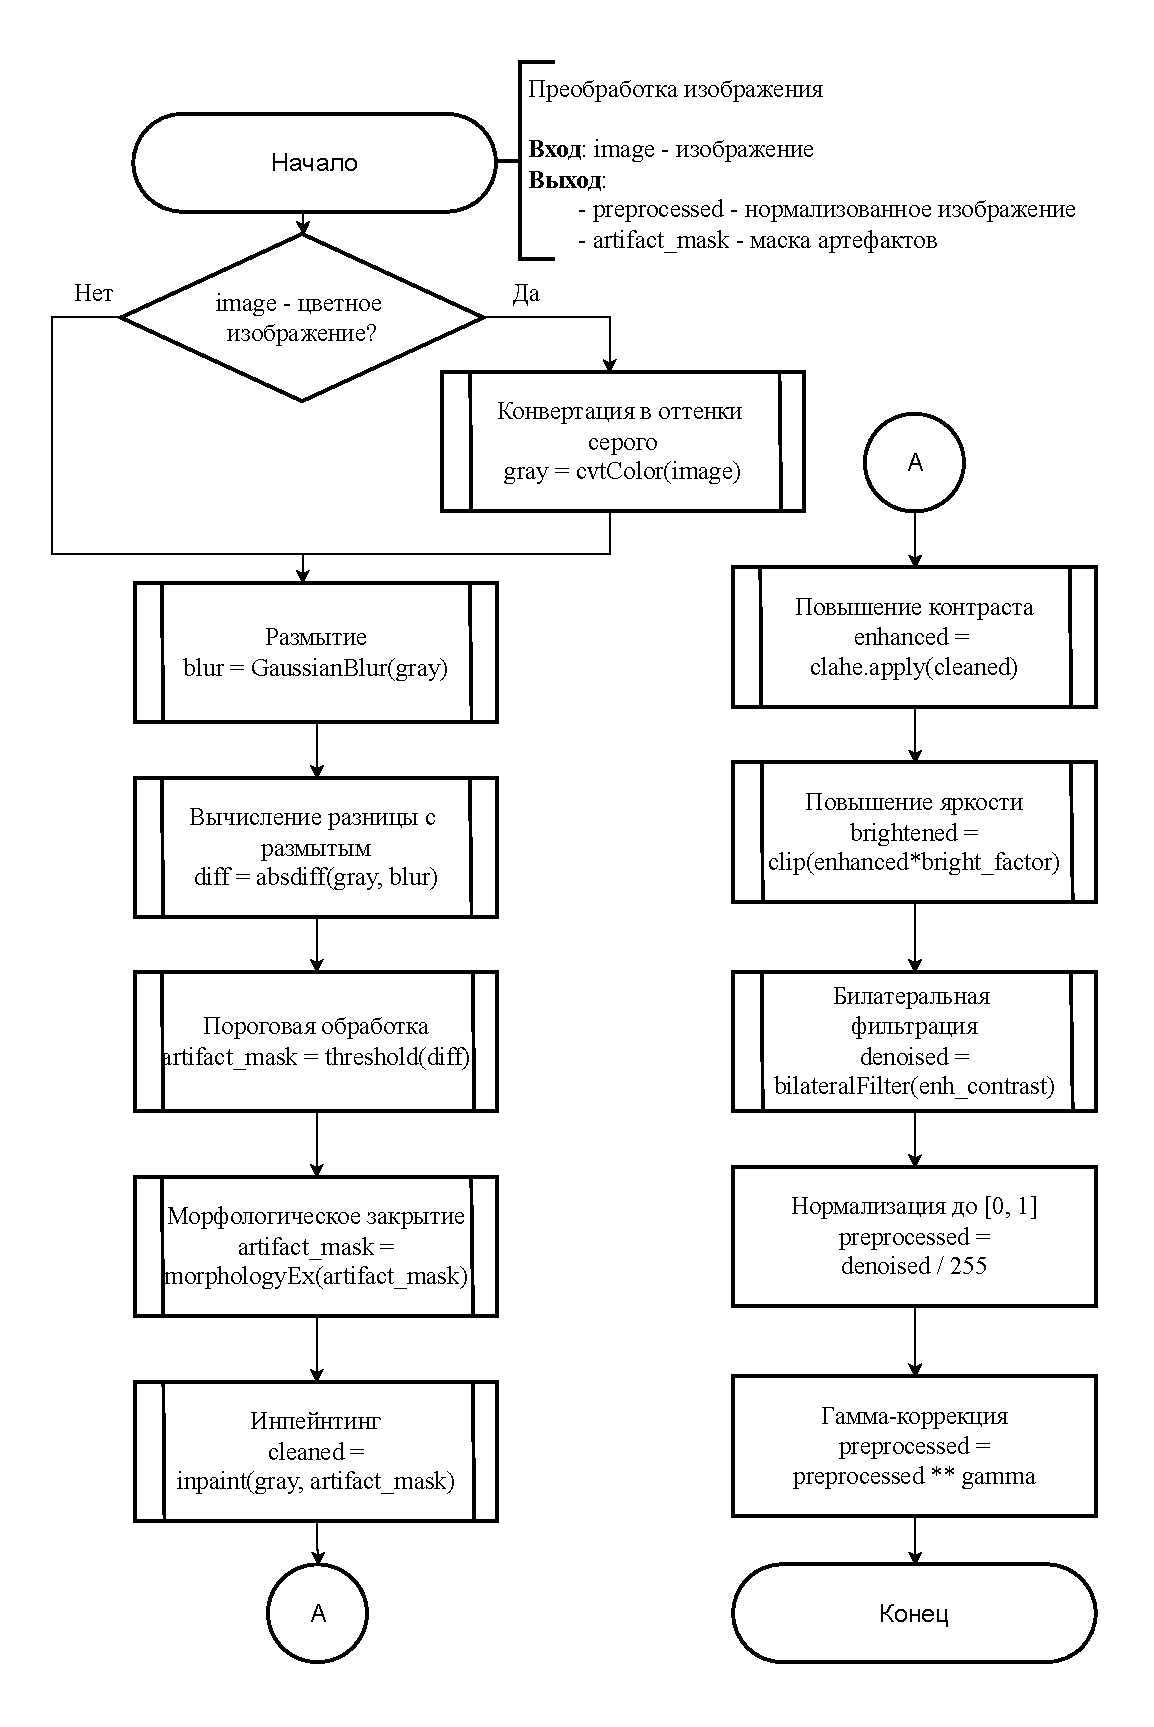
\includegraphics[scale=0.7]{img/preobr}
    \caption{Преобработка изображения}
    \label{preobr}
\end{figure}


Рисунок~\ref{reconstr} иллюстрирует основной алгоритм извлечения глубины, который объединяет нейросетевой метод для первичной оценки глубины с последующим уточнением деталей.

\begin{figure}[H]
    \centering
    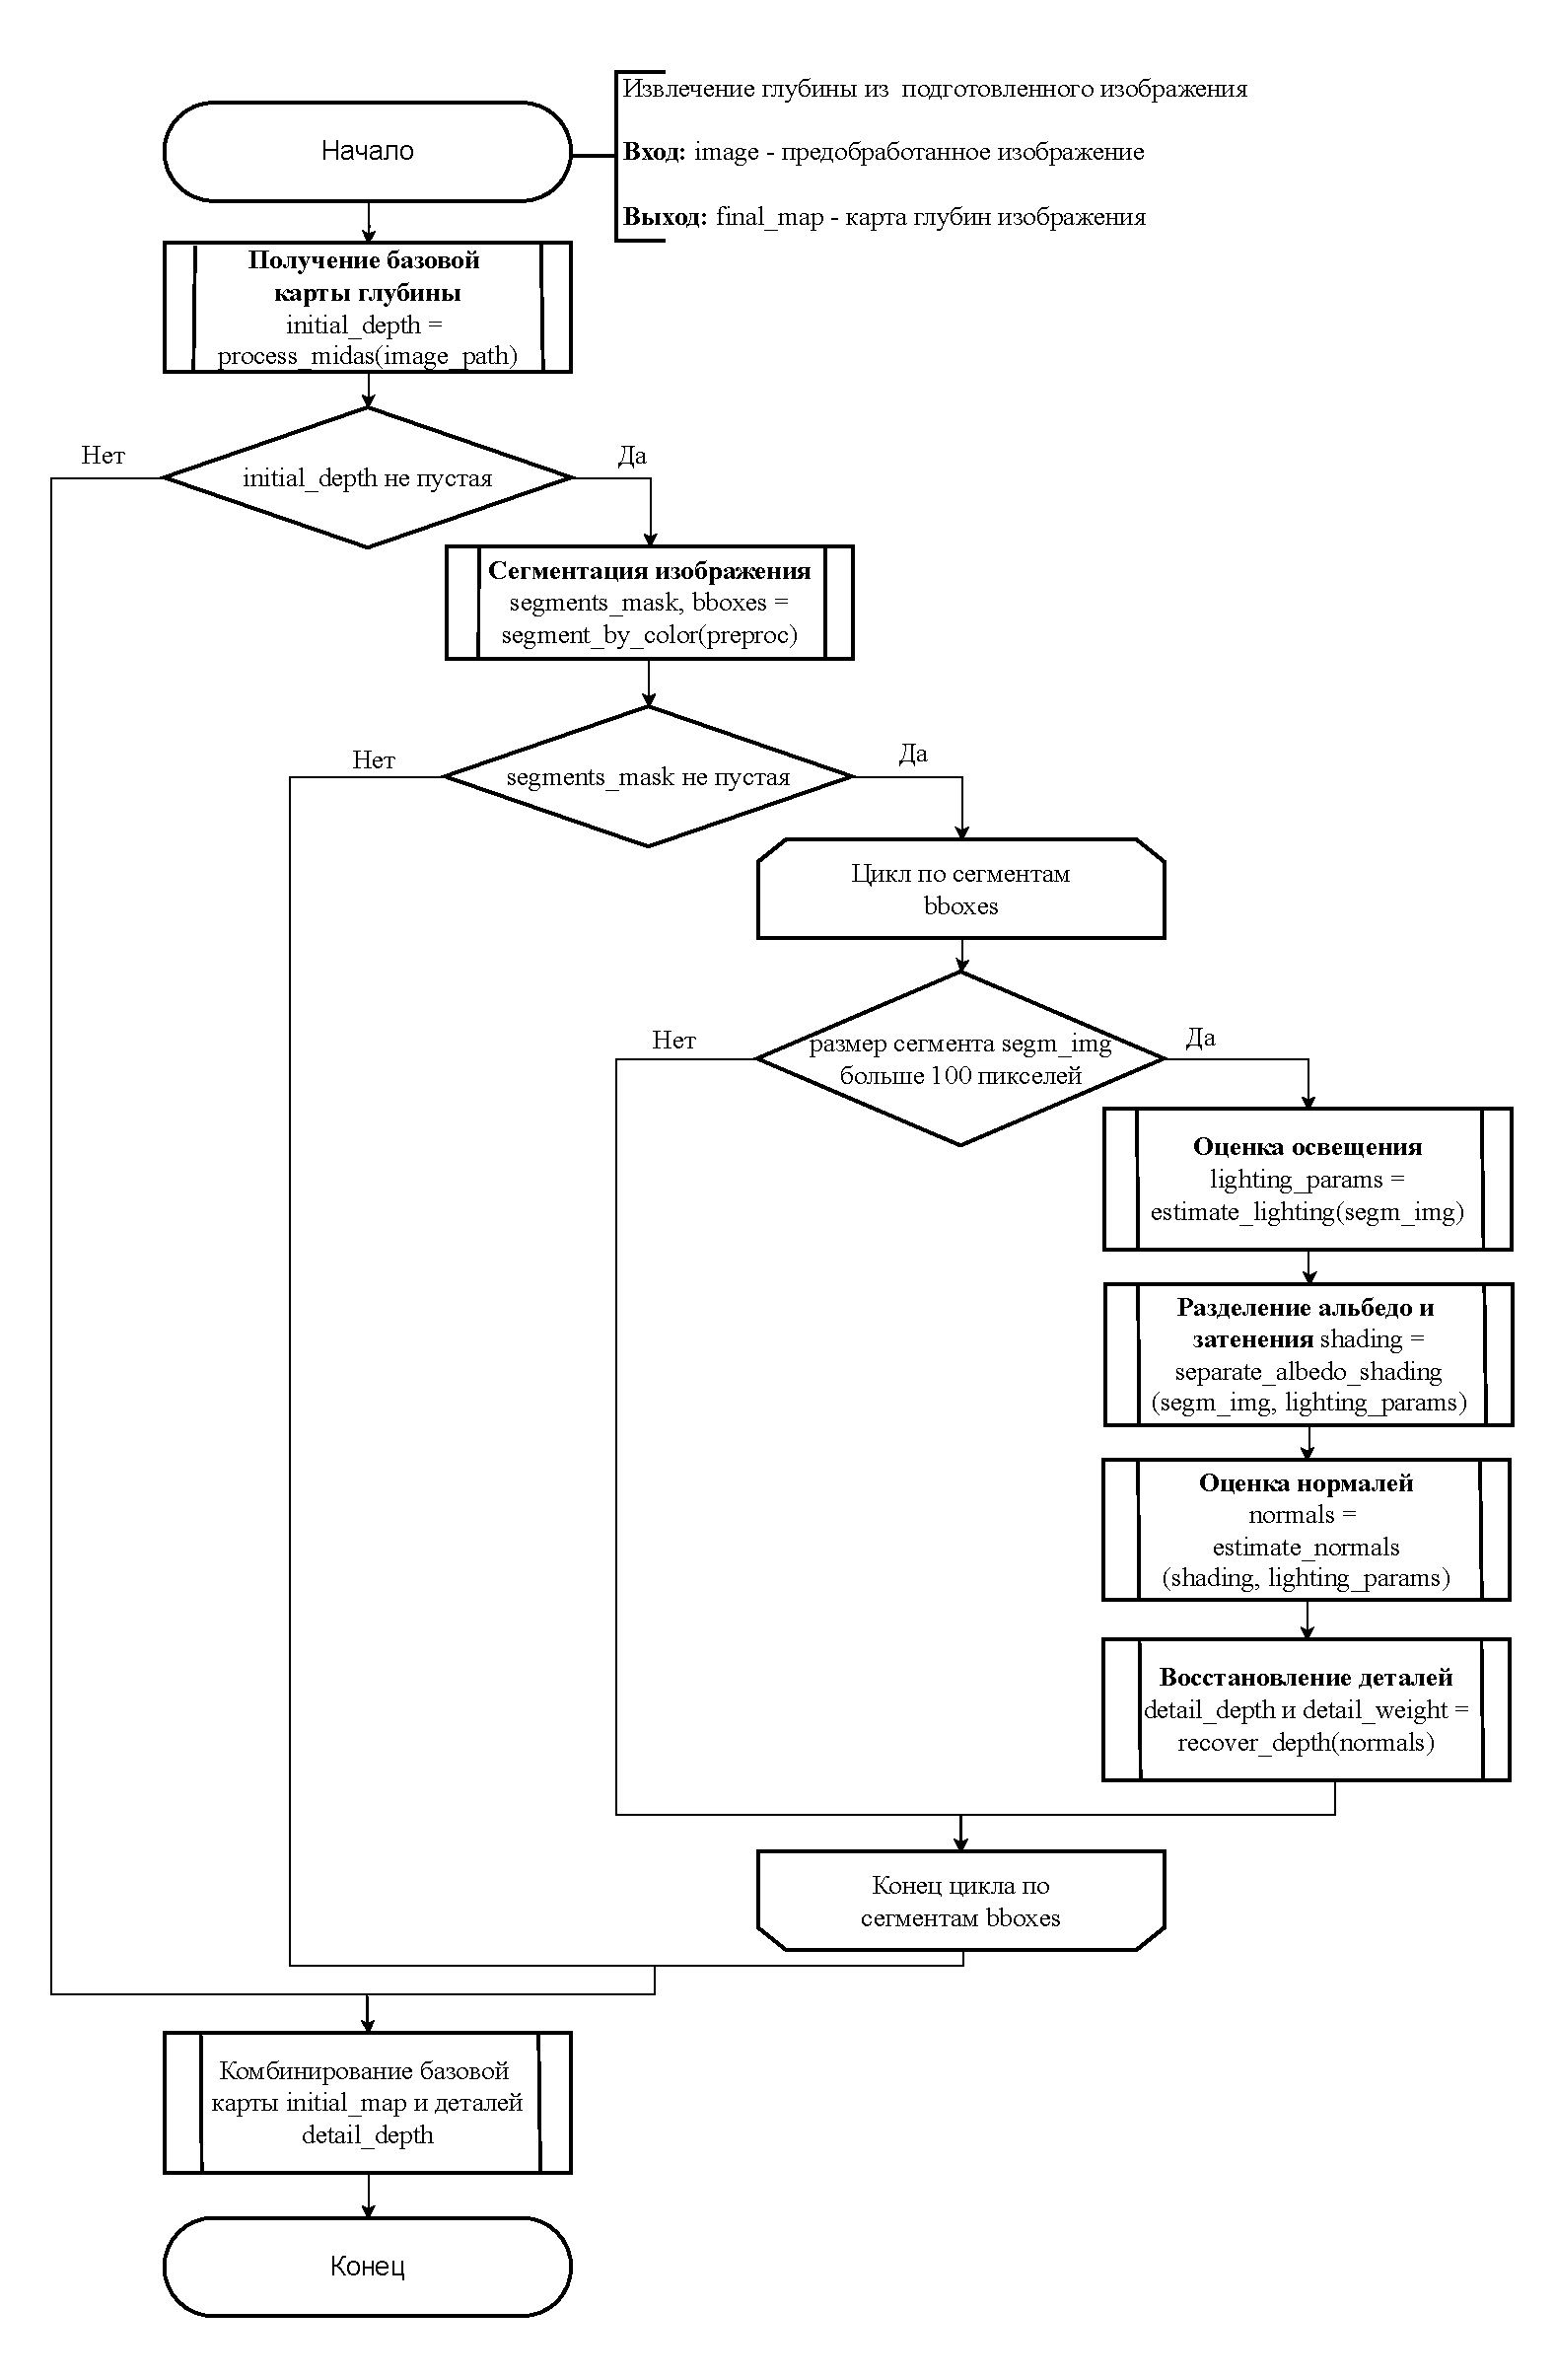
\includegraphics[scale=0.6]{img/reconstr}
    \caption{Извлечение глубины из подготовленного изображения}
    \label{reconstr}
\end{figure}

Схема на рисунке~\ref{segmentation} отражает процесс сегментации изображения, позволяющий выделить различные объекты сцены для их дальнейшей раздельной обработки методом Shape From Shading.

\begin{figure}[H]
    \centering
    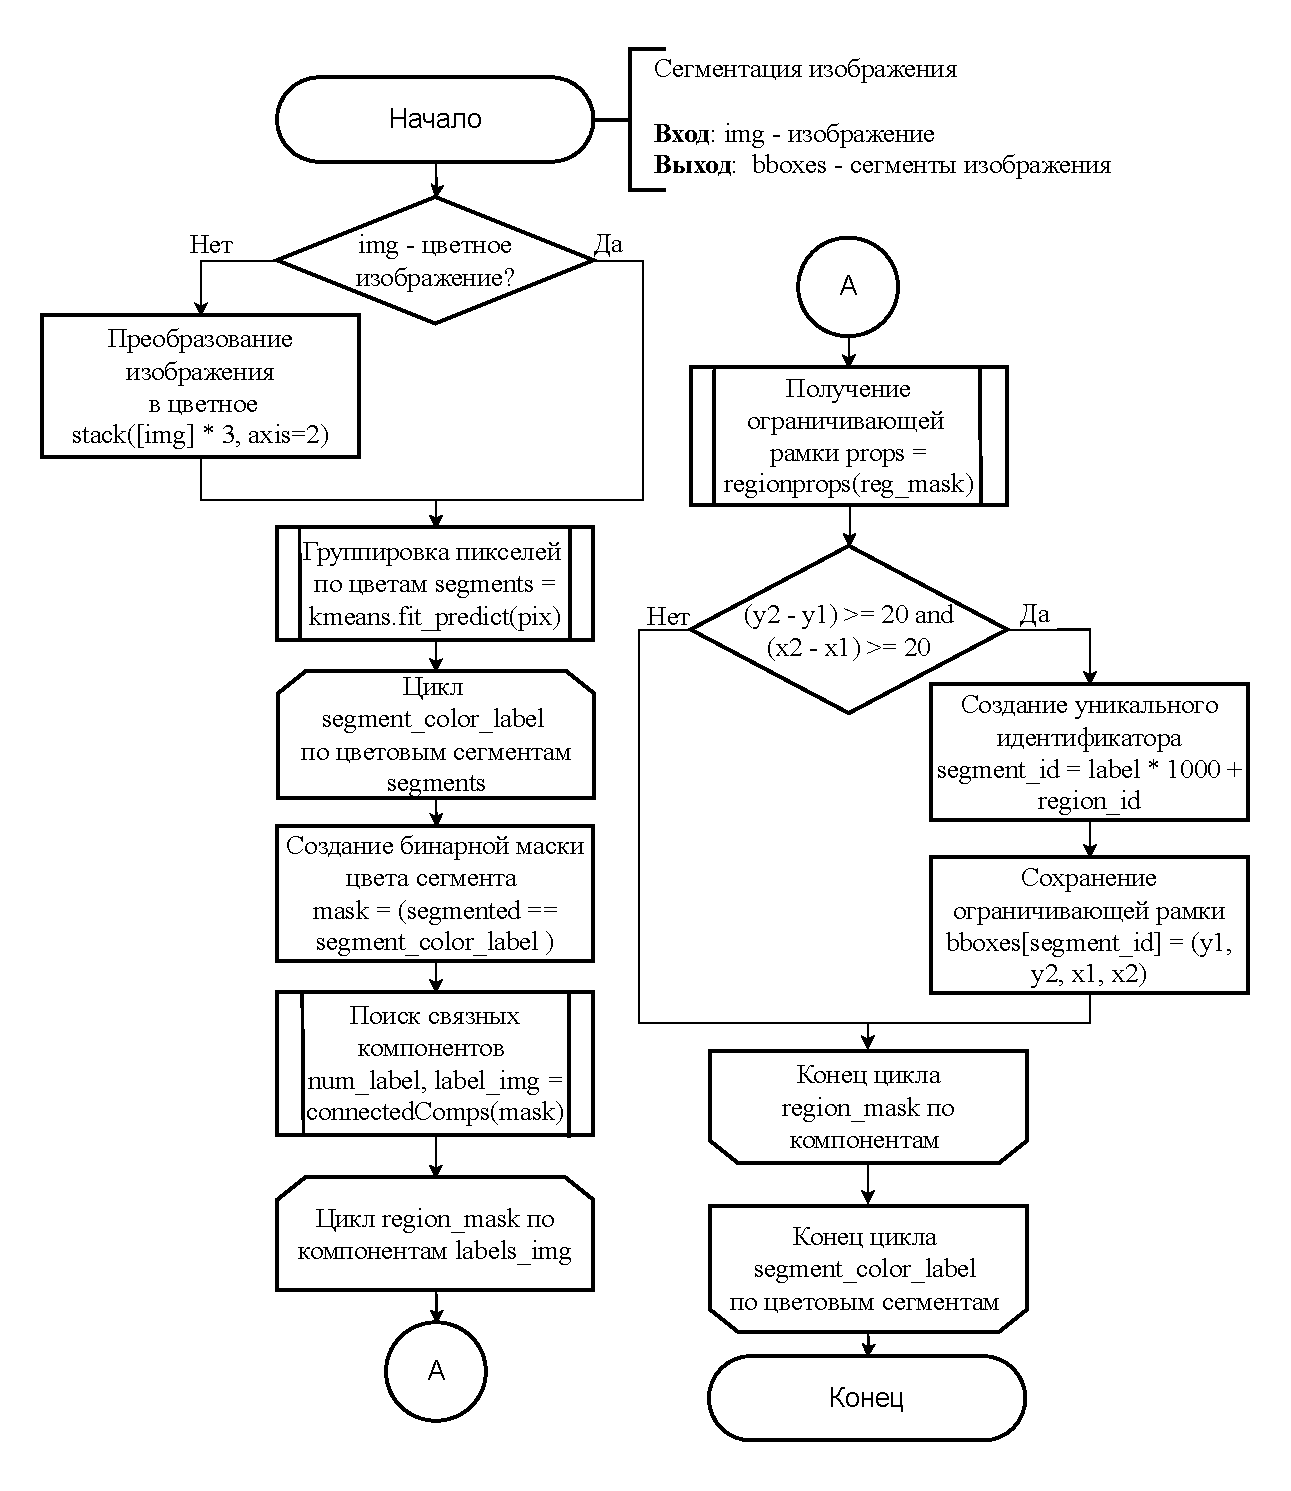
\includegraphics[scale=0.7]{img/segmentation}
    \caption{Сегментация изображения}
    \label{segmentation}
\end{figure}

На рисунке~\ref{light} представлен алгоритм оценки параметров освещения сцены, необходимых для корректного применения метода Shape from Shading.

\begin{figure}[H]
    \centering
    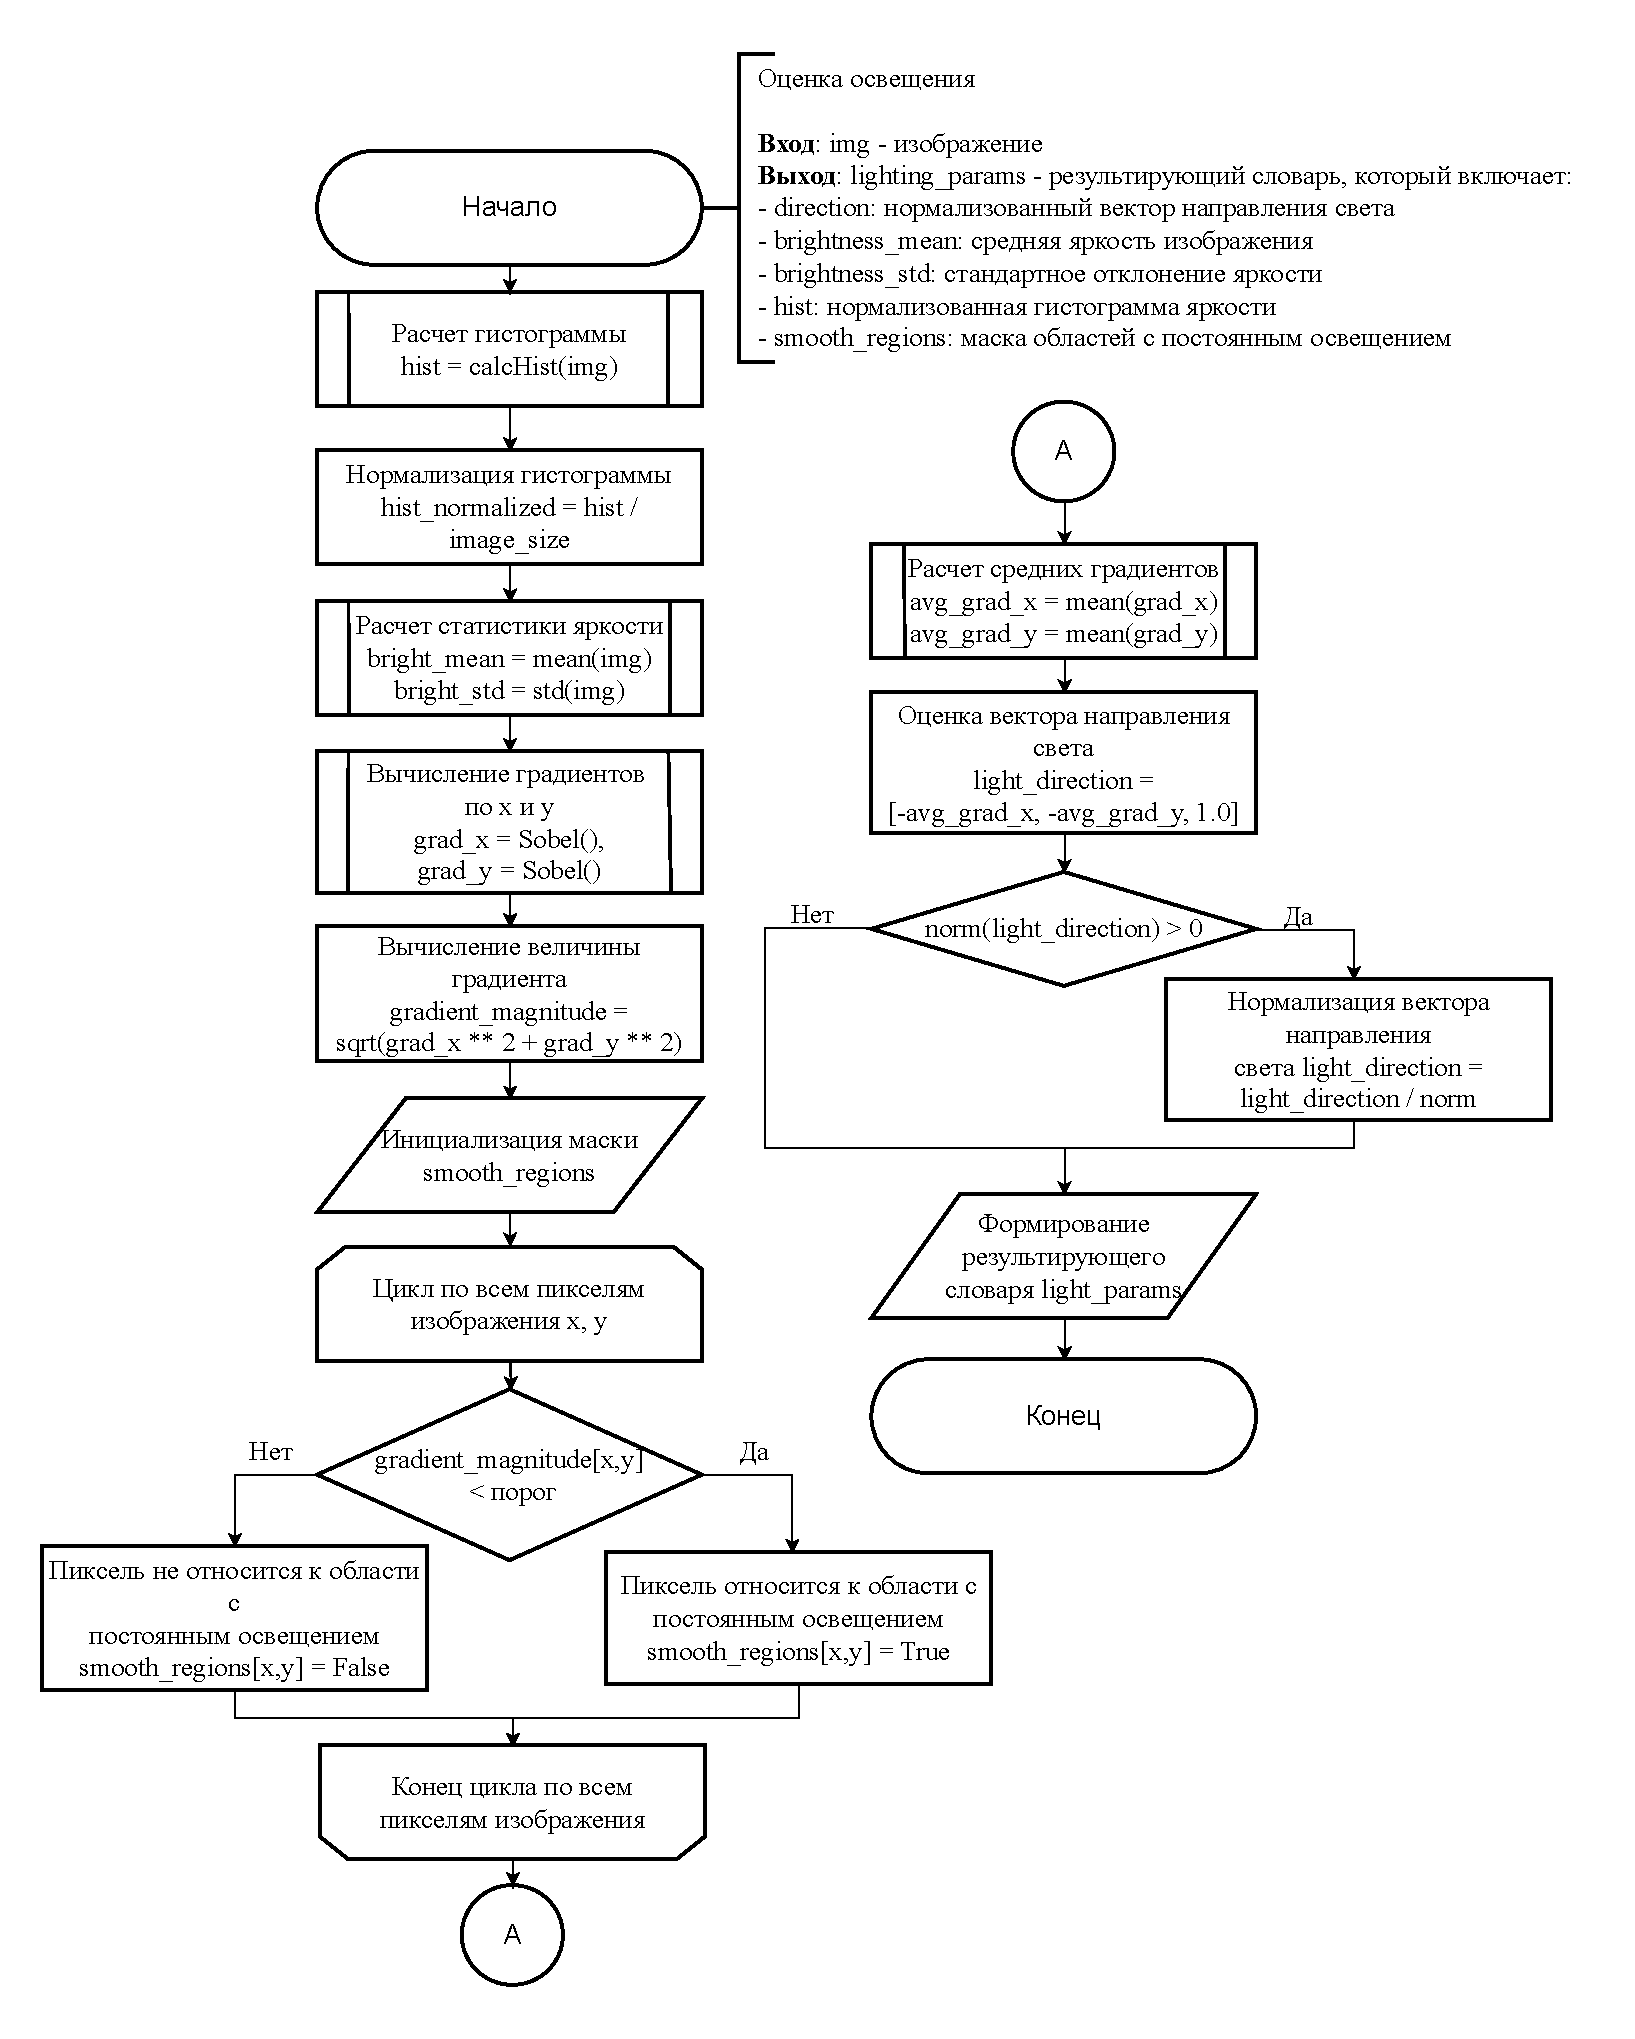
\includegraphics[scale=0.6]{img/light}
    \caption{Оценка освещения}
    \label{light}
\end{figure}

Рисунок~\ref{albedo} демонстрирует процесс разделения альбедо и затенения метода Shape from Shading, позволяющий отделить собственные цвета поверхностей от эффектов освещения.

\begin{figure}[H]
    \centering
    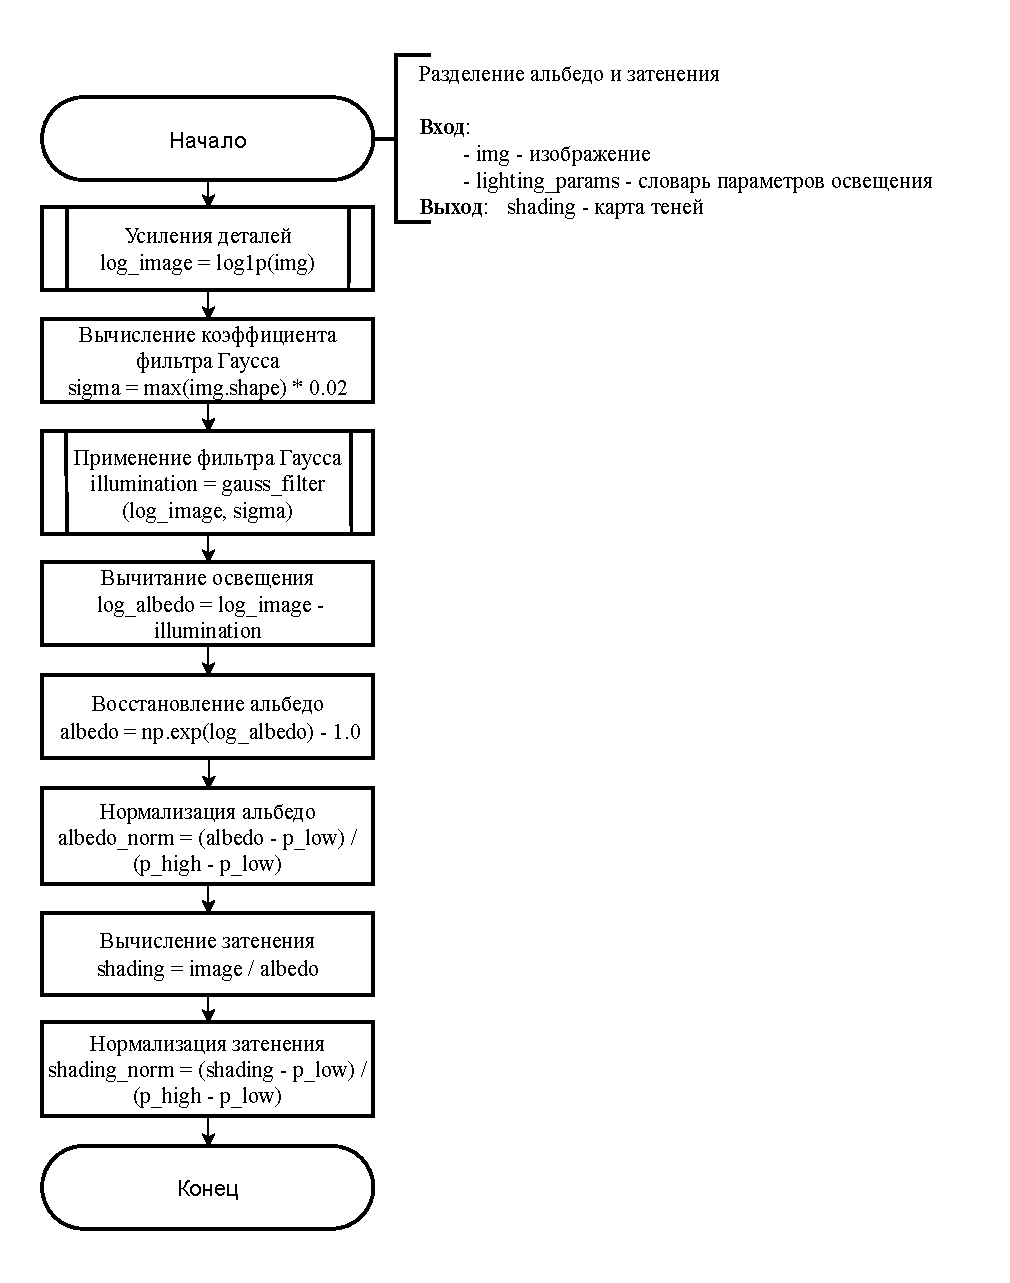
\includegraphics[scale=0.9]{img/albedo}
    \caption{Разделение альбедо и затенения}
    \label{albedo}
\end{figure}

Схема на рисунке~\ref{normals} описывает алгоритм вычисления нормалей к поверхности на основе полученного разделения альбедо и затенения.

\begin{figure}[H]
    \centering
    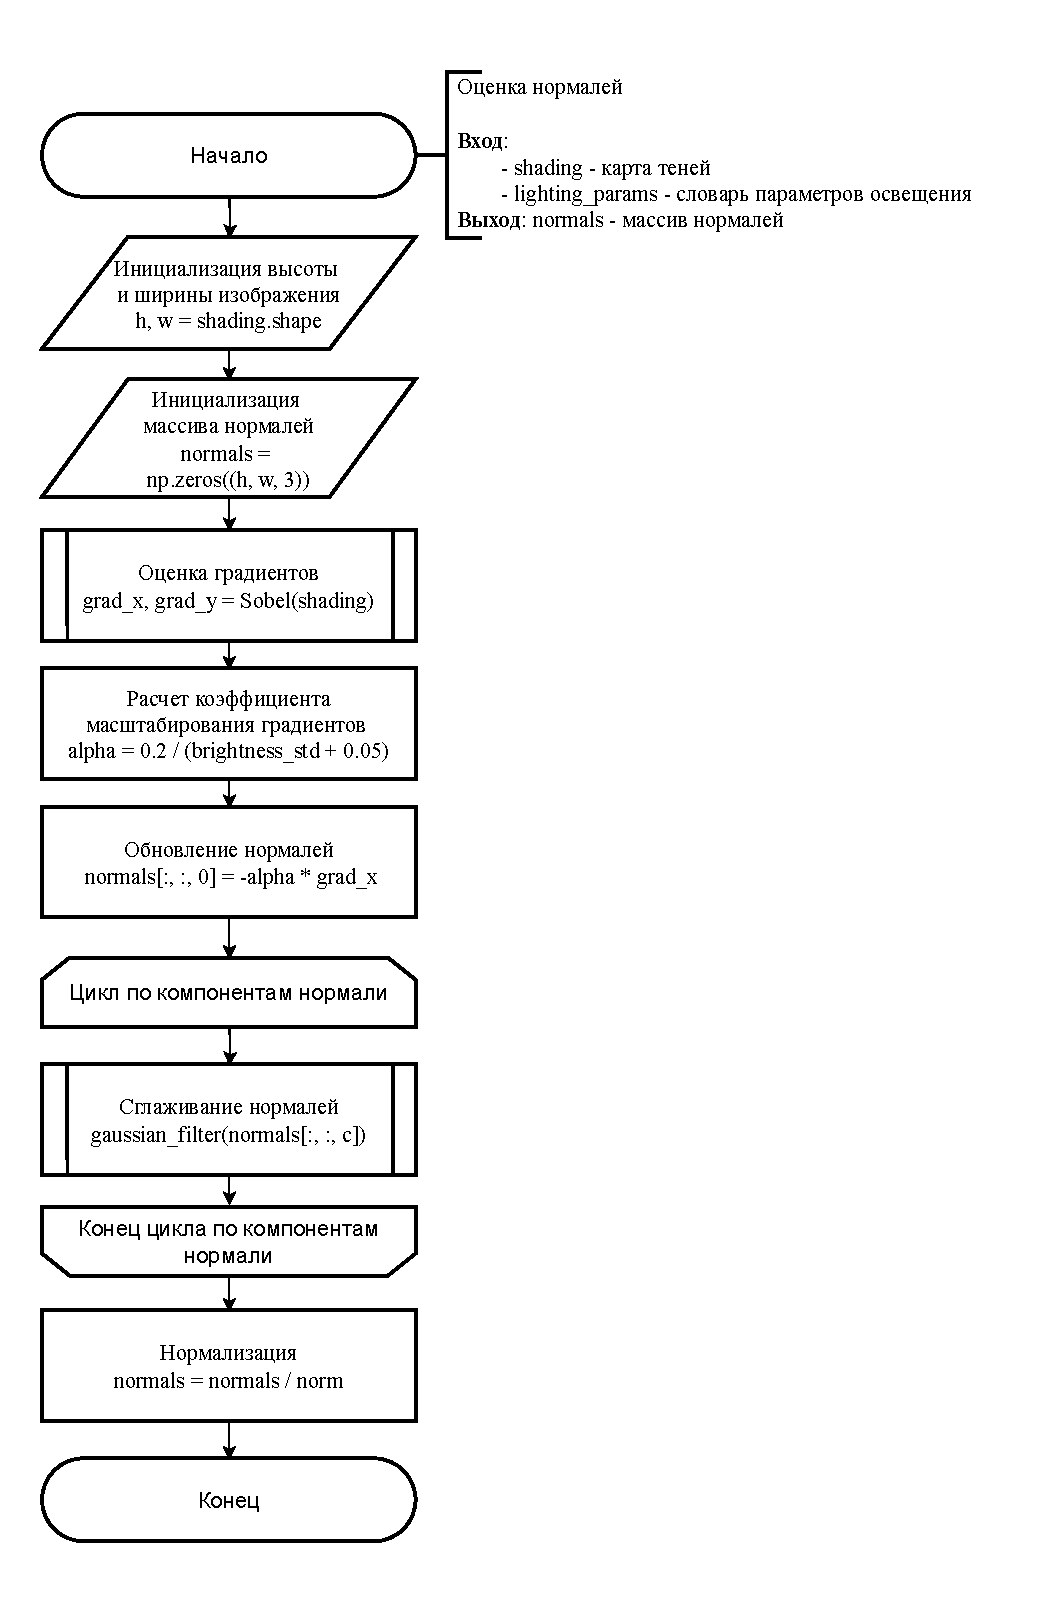
\includegraphics[scale=0.8]{img/normals}
    \caption{Оценка нормалей}
    \label{normals}
\end{figure}

Заключительный этап обработки представлен на рисунке~\ref{depth} --- алгоритм интеграции поля нормалей для получения итоговой карты глубин с высоким уровнем детализации поверхностей.

\begin{figure}[H]
    \centering
    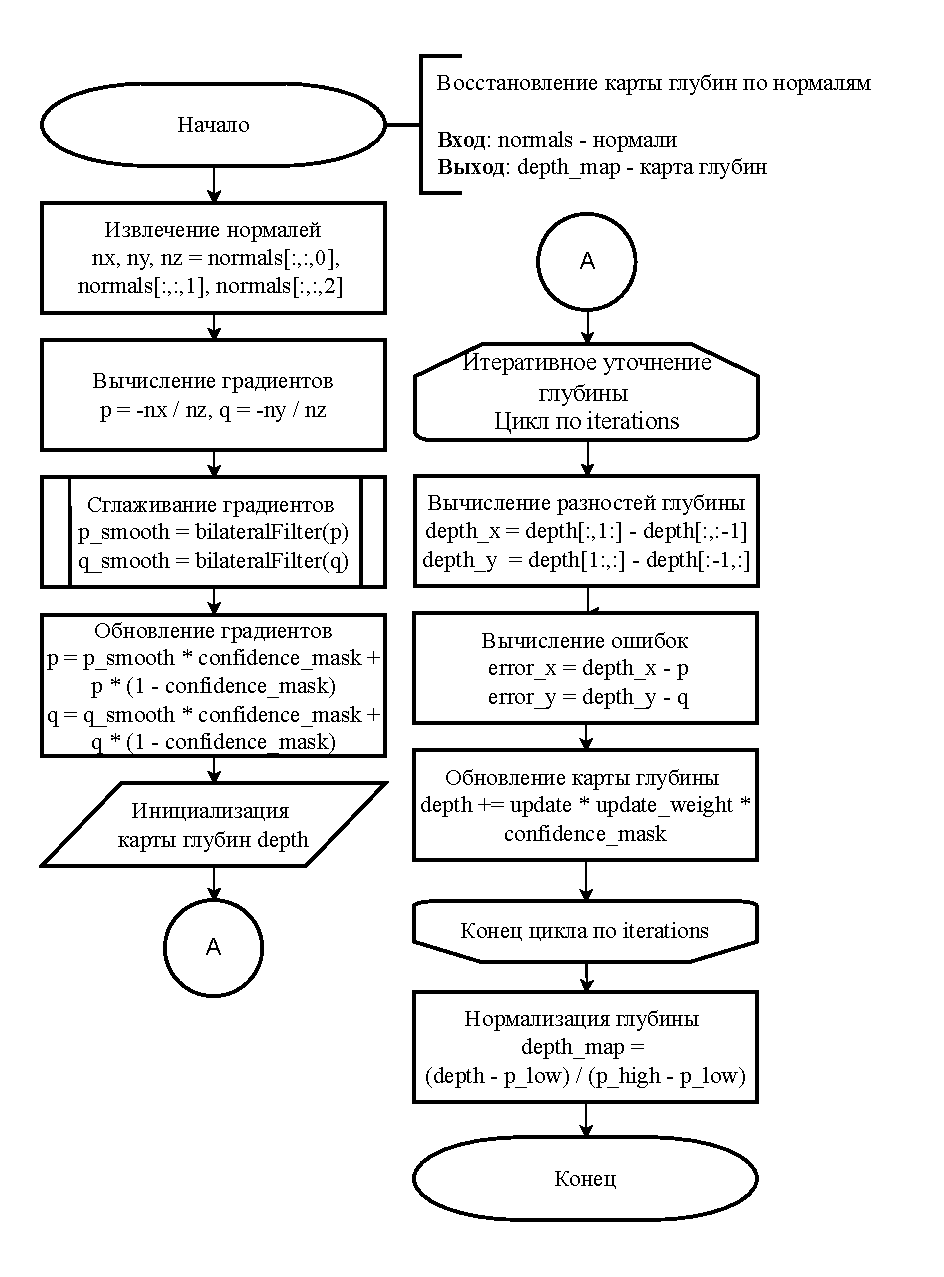
\includegraphics[scale=0.75]{img/depth}
    \caption{Восстановление карты глубин по нормалям}
    \label{depth}
\end{figure}

% TODO Надо добавить диаграмму компонентов разрабатываемого ПО?

\section*{Вывод}

В конструкторском разделе представлена детальная структура разработанного гибридного метода восстановления трехмерной информации из архивных фотографий.

Представленные схемы алгоритмов являются основой для последующей программной реализации метода, которая будет рассмотрена в технологическом разделе работы.

    \chapter{Технологический раздел}

Технологический раздел посвящен практической реализации гибридного метода восстановления глубины из монокулярных изображений.
В данном разделе рассматриваются ключевые аспекты программной реализации и тестирования разработанного решения.

Особое внимание уделяется обоснованию выбора программных средств и библиотек, необходимых для эффективной реализации алгоритмов.

Для объективной оценки качества реконструкции будут формализованы метрики: MAE, RMSE, REL и точность δ, позволяющие количественно оценивать эффективность метода на разных типах изображений.

\section{Выбор программных средств}

Для реализации методов восстановления глубины из монокулярных изображений был выбран язык программирования Python.
Этот выбор обусловлен наличием в его экосистеме всех необходимых библиотек и инструментов для комплексного решения поставленной задачи.

% TODO добавить ссылки на источники

\begin{enumerate}
    \item \textbf{Библиотеки обработки изображений:} OpenCV~\cite{opencv_library}, scikit-image~\cite{van2014scikit} и PIL/Pillow~\cite{clark2015pillow} — обеспечивают функционал для эффективной предобработки архивных фотографий, включая фильтрацию, сегментацию и работу с различными форматами файлов.
    \item \textbf{Библиотеки машинного обучения:} PyTorch~\cite{paszke2019pytorch}, TensorFlow/Keras~\cite{abadi2016tensorflow} и scikit-learn~\cite{pedregosa2011scikit} — предоставляют инструменты для применения предобученной модели MiDaS для оценки глубины, что исключает необходимость обучения собственной нейронной сети и повышает эффективность разработки.
    \item \textbf{Библиотеки научных вычислений:} NumPy~\cite{harris2020array}, SciPy~\cite{virtanen2020scipy}, Matplotlib~\cite{hunter2007matplotlib} и Open3D~\cite{zhou2018open3d} — обеспечивают эффективную работу с многомерными массивами, методы оптимизации, визуализацию результатов и обработку трехмерных данных.
\end{enumerate}

Таким образом, совокупность доступных в Python библиотек делает его достаточным инструментом для решения всех аспектов задачи восстановления глубины, включая предобработку данных, использование готовой модели MiDaS и визуализацию результатов.

\section{Описание входных и выходных данных}

Входными данными для алгоритмов восстановления глубины являются монокулярные цветные фотографии в различных форматах (JPEG, PNG, TIFF).

Результатом работы алгоритмов восстановления глубины являются карта глубин в виде одноканальных изображений, где:

\begin{itemize}
    \item значение пикселя соответствует относительному расстоянию от камеры (меньшие значения — ближе к камере);
    \item диапазон значений нормализован от 0 до 1 (или от 0 до 255 для 8-битных изображений);
    \item разрешение карты глубины соответствует разрешению входного изображения.
\end{itemize}



    \chapter{Технологический раздел}

Технологический раздел посвящен практической реализации гибридного метода восстановления глубины из монокулярных изображений.
В данном разделе рассматриваются ключевые аспекты программной реализации и тестирования разработанного решения.

Особое внимание уделяется обоснованию выбора программных средств и библиотек, необходимых для эффективной реализации алгоритмов.

Для объективной оценки качества реконструкции будут формализованы метрики: MAE, RMSE, REL и точность δ, позволяющие количественно оценивать эффективность метода на разных типах изображений.

\section{Выбор программных средств}

Для реализации методов восстановления глубины из монокулярных изображений был выбран язык программирования Python.
Этот выбор обусловлен наличием в его экосистеме всех необходимых библиотек и инструментов для комплексного решения поставленной задачи.

% TODO добавить ссылки на источники

\begin{enumerate}
    \item \textbf{Библиотеки обработки изображений:} OpenCV~\cite{opencv_library}, scikit-image~\cite{van2014scikit} и PIL/Pillow~\cite{clark2015pillow} — обеспечивают функционал для эффективной предобработки архивных фотографий, включая фильтрацию, сегментацию и работу с различными форматами файлов.
    \item \textbf{Библиотеки машинного обучения:} PyTorch~\cite{paszke2019pytorch}, TensorFlow/Keras~\cite{abadi2016tensorflow} и scikit-learn~\cite{pedregosa2011scikit} — предоставляют инструменты для применения предобученной модели MiDaS для оценки глубины, что исключает необходимость обучения собственной нейронной сети и повышает эффективность разработки.
    \item \textbf{Библиотеки научных вычислений:} NumPy~\cite{harris2020array}, SciPy~\cite{virtanen2020scipy}, Matplotlib~\cite{hunter2007matplotlib} и Open3D~\cite{zhou2018open3d} — обеспечивают эффективную работу с многомерными массивами, методы оптимизации, визуализацию результатов и обработку трехмерных данных.
\end{enumerate}

Таким образом, совокупность доступных в Python библиотек делает его достаточным инструментом для решения всех аспектов задачи восстановления глубины, включая предобработку данных, использование готовой модели MiDaS и визуализацию результатов.

\section{Описание входных и выходных данных}

Входными данными для алгоритмов восстановления глубины являются монокулярные цветные фотографии в различных форматах (JPEG, PNG, TIFF).

Результатом работы алгоритмов восстановления глубины являются карта глубин в виде одноканальных изображений, где:

\begin{itemize}
    \item значение пикселя соответствует относительному расстоянию от камеры (меньшие значения — ближе к камере);
    \item диапазон значений нормализован от 0 до 1 (или от 0 до 255 для 8-битных изображений);
    \item разрешение карты глубины соответствует разрешению входного изображения.
\end{itemize}


\section{Реализация методов}

% TODO добавить Листингиииииииииииии

В листинге~\ref{lst:preproc} представлен код предварительной обработки входного изображения, включающий методы шумоподавления, нормализации освещения и коррекции артефактов, характерных для архивных фотографий.

\begin{center}
    \captionsetup{justification=raggedright,singlelinecheck=off}
    \begin{lstlisting}[label=lst:preproc,caption=Предварительная обработка изображения]
        import cv2
        import numpy as np


        def preprocess_archival_photo(image_path, brightness_boost=1.5, contrast_boost=1.2):
            if isinstance(image_path, str):
                image = cv2.imread(image_path)
                if image is not None and len(image.shape) == 3:
                    image = cv2.cvtColor(image, cv2.COLOR_BGR2RGB)
            else:
                image = image_path.copy()

            # Проверяем, является ли изображение цветным или оттенков серого
            if len(image.shape) == 3:
                gray = cv2.cvtColor(image, cv2.COLOR_RGB2GRAY)
            else:
                gray = image.copy()

            # Выявление и маскирование дефектов
            blur = cv2.GaussianBlur(gray, (5, 5), 0)
            diff = cv2.absdiff(gray, blur)
            _, artifact_mask = cv2.threshold(diff, 25, 255, cv2.THRESH_BINARY)

            kernel = np.ones((3, 3), np.uint8)
            artifact_mask = cv2.morphologyEx(artifact_mask, cv2.MORPH_CLOSE, kernel)
            artifact_mask = cv2.dilate(artifact_mask, kernel, iterations=1)

            # Инпейнтинг для удаления дефектов
            cleaned = cv2.inpaint(gray, artifact_mask.astype(np.uint8), 3, cv2.INPAINT_TELEA)

            # Повышение контраста
            clahe = cv2.createCLAHE(clipLimit=2.0, tileGridSize=(8, 8))
            enhanced = clahe.apply(cleaned)

            # Повышение яркости
            mean_brightness = np.mean(enhanced)
            target_brightness = 80

            brightness_factor = min((target_brightness / (mean_brightness + 1e-6)), brightness_boost)
            brightened = np.clip(enhanced * brightness_factor, 0, 255).astype(np.uint8)

            # Улучшение контраста
            alpha = min(contrast_boost, 1.1)
            beta = 128 * (1 - alpha)
            enhanced_contrast = np.clip(alpha * brightened + beta, 0, 255).astype(np.uint8)

            # Билатеральная фильтрация для сохранения краев при устранении шума
            denoised = cv2.bilateralFilter(enhanced_contrast, 7, 25, 25)

            # Нормализация до [0, 1]
            preprocessed = denoised.astype(np.float32) / 255.0

            # Гамма-коррекция для улучшения контраста в средних тонах
            gamma = 1.1
            preprocessed = np.power(preprocessed, gamma)

            return preprocessed, artifact_mask
    \end{lstlisting}
\end{center}

Листинг~\ref{lst:depth_extract} иллюстрирует основной алгоритм извлечения глубины, который объединяет нейросетевой метод для первичной оценки глубины с последующим уточнением деталей.

\begin{center}
    \captionsetup{justification=raggedright,singlelinecheck=off}
    \begin{lstlisting}[label=lst:depth_extract,caption=Извлечение глубины из подготовленного изображения]
        import os
import sys
import numpy as np
import cv2
import time

from scipy.ndimage import gaussian_filter, sobel

# Добавляем путь к директории code
sys.path.append(os.path.dirname(os.path.dirname(os.path.abspath(__file__))))

# Изменим импорты, чтобы они указывали на директории внутри code
from preprocessing.image_cleaner import preprocess_archival_photo
from preprocessing.segmentation import segment_by_color
from reconstruction.lighting import estimate_lighting
from reconstruction.albedo_shading import separate_albedo_shading
from reconstruction.normals import estimate_normals
from reconstruction.depth import recover_depth
from reconstruction.midas_depth import estimate_depth_midas
from postprocessing.refinement import postprocess_depth

class ArchivalDepthReconstruction:
    def __init__(self, iterations=200, lambda_smooth=0.15, regularization_weight=0.3,
                 brightness_boost=1.5, contrast_boost=1.2, n_color_segments=6,
                 method="segmentation", midas_model="MiDaS_small"):
        self.iterations = iterations
        self.lambda_smooth = lambda_smooth
        self.regularization_weight = regularization_weight
        self.brightness_boost = brightness_boost
        self.contrast_boost = contrast_boost
        self.n_color_segments = n_color_segments
        self.method = method
        self.midas_model = midas_model

    def process_hybrid(self, image_path):

        # Шаг 1: Получение базовой карты глубины
        print("Получение базовой карты глубины через MiDaS...")
        midas_results = self.process_midas(image_path)
        base_depth = midas_results['depth_map']
        preprocessed = midas_results['preprocessed']
        artifact_mask = np.zeros_like(preprocessed, dtype=np.uint8)

        # Шаг 2: Сегментация изображения
        print("Сегментация изображения для детализации...")
        segments_mask, bboxes = segment_by_color(
            preprocessed,
            self.n_color_segments
        )

        # Шаг 3: Инициализация карт деталей
        detail_depth = np.zeros_like(base_depth)
        detail_weight = np.zeros_like(base_depth)

        # Шаг 4: Цикл по сегментам
        print("Детализация каждого сегмента...")
        for segment_id, bbox in bboxes.items():
            y1, y2, x1, x2 = bbox

            segment_mask = (segments_mask[y1:y2, x1:x2] == segment_id).astype(np.float32)

            # Пропускаем слишком маленькие сегменты
            if np.sum(segment_mask) < 100:
                continue

            segment_img = preprocessed[y1:y2, x1:x2].copy()
            segment_base_depth = base_depth[y1:y2, x1:x2].copy()

            # Оценка условий освещения
            lighting_params = estimate_lighting(segment_img)

            # Разделение альбедо и затенения
            albedo, shading = separate_albedo_shading(segment_img, lighting_params)

            # Оценка нормалей поверхности
            normals, confidence_mask = estimate_normals(shading, lighting_params)

            # Восстановление деталей
            segment_details = recover_depth(
                normals,
                confidence_mask,
                iterations=self.iterations // 2,
                initial_depth=segment_base_depth
            )

            segment_weight = confidence_mask * np.abs(sobel(segment_img, axis=0)) * np.abs(sobel(segment_img, axis=1))
            segment_weight = gaussian_filter(segment_weight, sigma=1.0)
            if np.max(segment_weight) > 0:
                segment_weight = segment_weight / np.max(segment_weight)
            detail_depth[y1:y2, x1:x2] += segment_details * segment_mask * segment_weight
            detail_weight[y1:y2, x1:x2] += segment_mask * segment_weight

        # Шаг 5: Комбинация базовой карты и деталей
        detail_weight = np.maximum(detail_weight, 1e-6)
        detail_depth = detail_depth / detail_weight

        alpha_base = 0.7
        alpha_map = alpha_base - (detail_weight * 0.4)
        alpha_map = np.clip(alpha_map, 0.3, 0.9)

        final_depth = alpha_map * base_depth + (1 - alpha_map) * detail_depth


        # Формирование результатов
        results = {
            'preprocessed': preprocessed,
            'segments_mask': segments_mask,
            'depth_map': base_depth,
            'detail_depth': detail_depth,
            'detail_weight': detail_weight,
            'final_depth': final_depth,
            'bboxes': bboxes,
        }

        return results
    \end{lstlisting}
\end{center}

В листинге~\ref{lst:segmentation} представлен код сегментации изображения, позволяющий выделить различные объекты сцены для их дальнейшей раздельной обработки методом Shape From Shading.

\begin{center}
    \captionsetup{justification=raggedright,singlelinecheck=off}
    \begin{lstlisting}[label=lst:segmentation,caption=Сегментация изображения]
        import cv2
import numpy as np
from skimage.measure import regionprops
from sklearn.cluster import KMeans


def segment_by_color(img, n_color_segments=6):
    # Преобразование изображения в цветное
    if len(img.shape) == 2:
        image_for_cluster = np.stack([img] * 3, axis=2)
    else:
        image_for_cluster = img.copy()

    pixels = image_for_cluster.reshape(-1, 3)

    # Группировка пикселей по цветам
    kmeans = KMeans(n_clusters=n_color_segments, random_state=42, n_init=10)
    labels = kmeans.fit_predict(pixels)

    segmented = labels.reshape(img.shape[:2])

    h, w = segmented.shape[:2]
    bboxes = {}

    # Цикл по цветовым сегментам
    for label in range(n_color_segments):
        # Создание бинарной маски для текущего цвета
        mask = (segmented == label).astype(np.uint8)

        # Поиск связных компонентов
        num_labels, labels_img = cv2.connectedComponents(mask)

        for region_id in range(1, num_labels):
            region_mask = (labels_img == region_id).astype(np.uint8)

            # Получение прямоугольной ограничивающей рамки
            props = regionprops(region_mask)
            if not props:
                continue

            y1, x1, y2, x2 = props[0].bbox

            margin = 5
            y1 = max(0, y1 - margin)
            y2 = min(h, y2 + margin)
            x1 = max(0, x1 - margin)
            x2 = min(w, x2 + margin)

            # Если область слишком маленькая, она пропускается
            if (y2 - y1) < 20 or (x2 - x1) < 20:
                continue

            # Создание уникального идентификатора для этого прямоугольного сегмента
            segment_id = label * 1000 + region_id

            segmented[y1:y2, x1:x2][region_mask[y1:y2, x1:x2] > 0] = segment_id

            # Сохранение ограничивающей рамки
            bboxes[segment_id] = (y1, y2, x1, x2)

    return segmented, bboxes

    \end{lstlisting}
\end{center}

Листинг~\ref{lst:light_estimation} представляет реализацию алгоритма оценки параметров освещения сцены, необходимых для корректного применения метода Shape from Shading.

\begin{center}
    \captionsetup{justification=raggedright,singlelinecheck=off}
    \begin{lstlisting}[label=lst:light_estimation,caption=Оценка освещения]
import cv2
import numpy as np


def estimate_lighting(image):
    hist = cv2.calcHist([image * 255], [0], None, [256], [0, 256])
    hist_normalized = hist / (image.shape[0] * image.shape[1])
    brightness_mean = np.mean(image)
    brightness_std = np.std(image)

    # Вычисляем градиенты
    grad_x = cv2.Sobel(image, cv2.CV_32F, 1, 0, ksize=5)
    grad_y = cv2.Sobel(image, cv2.CV_32F, 0, 1, ksize=5)
    gradient_magnitude = np.sqrt(grad_x ** 2 + grad_y ** 2)

    # Определяем области с постоянным освещением
    smooth_regions = gradient_magnitude < np.percentile(gradient_magnitude, 25)

    # Оцениваем направление света по градиентам
    avg_grad_x = np.mean(grad_x)
    avg_grad_y = np.mean(grad_y)

    light_x = -avg_grad_x
    light_y = -avg_grad_y
    light_z = 1.0

    light_direction = np.array([light_x, light_y, light_z])
    norm = np.linalg.norm(light_direction)
    if norm > 0:
        light_direction = light_direction / norm

    lighting_params = {
        'direction': light_direction,
        'brightness_mean': brightness_mean,
        'brightness_std': brightness_std,
        'hist': hist_normalized,
        'smooth_regions': smooth_regions
    }

    return lighting_params

    \end{lstlisting}
\end{center}

В листинге~\ref{lst:albedo_separation} представлен код разделения альбедо и затенения метода Shape from Shading, позволяющий отделить собственные цвета поверхностей от эффектов освещения.

\begin{center}
    \captionsetup{justification=raggedright,singlelinecheck=off}
    \begin{lstlisting}[label=lst:albedo_separation,caption=Разделение альбедо и затенения]
# Содержимое файла albedo_separation.py
# Код разделения альбедо и затенения
    \end{lstlisting}
\end{center}

Листинг~\ref{lst:normals_estimation} содержит код вычисления нормалей к поверхности на основе полученного разделения альбедо и затенения.

\begin{center}
    \captionsetup{justification=raggedright,singlelinecheck=off}
    \begin{lstlisting}[label=lst:normals_estimation,caption=Оценка нормалей]
# Содержимое файла normals_estimation.py
# Код оценки нормалей
    \end{lstlisting}
\end{center}

Заключительный этап обработки представлен в листинге~\ref{lst:depth_integration} --- алгоритм интеграции поля нормалей для получения итоговой карты глубины с высоким уровнем детализации поверхностей.

\begin{center}
    \captionsetup{justification=raggedright,singlelinecheck=off}
    \begin{lstlisting}[label=lst:depth_integration,caption=Восстановление карты глубин по нормалям]
# Содержимое файла depth_integration.py
# Код восстановления карты глубин по нормалям
    \end{lstlisting}
\end{center}





\section{Метрики оценки качества реконструкции глубины}

% TODO добавить ссылки на источники

\subsection{Абсолютная средняя ошибка (MAE)}
\begin{equation}
\text{MAE} = \frac{1}{n} \sum_{i=1}^{n} |d_{i}^{\text{pred}} - d_{i}^{\text{gt}}|
\end{equation}

MAE представляет собой среднее абсолютное отклонение предсказанной глубины от эталонной. Эта метрика менее чувствительна к выбросам по сравнению с RMSE и позволяет выявлять систематические ошибки в предсказании глубины~\cite{zhang2025review}.

\subsection{Среднеквадратичная ошибка (RMSE)}
\begin{equation}
\text{RMSE} = \sqrt{\frac{1}{n} \sum_{i=1}^{n} (d_{i}^{\text{pred}} - d_{i}^{\text{gt}})^2}
\end{equation}

RMSE придаёт больший вес крупным ошибкам и является стандартной метрикой для оценки точности методов оценки глубины~\cite{vis3}. Благодаря своей чувствительности к выбросам, данная метрика эффективна при оценке методов, где критично минимизировать значительные отклонения.

\subsection{Относительная абсолютная ошибка (REL)}
\begin{equation}
\text{REL} = \frac{1}{n} \sum_{i=1}^{n} \frac{|d_{i}^{\text{pred}} - d_{i}^{\text{gt}}|}{d_{i}^{\text{gt}}}
\end{equation}

REL учитывает относительную величину ошибки, что особенно важно при работе с объектами, находящимися на разном расстоянии от камеры. Эта метрика предпочтительна при оценке качества реконструкции исторических объектов, где точная ш��ала глубины может быть неизвестна~\cite{zhang2025review}.

\subsection{Точность $\delta$}
\begin{equation}
\delta_{k} = \frac{1}{n} \sum_{i=1}^{n} \mathbb{I}\left[\max\left(\frac{d_{i}^{\text{pred}}}{d_{i}^{\text{gt}}}, \frac{d_{i}^{\text{gt}}}{d_{i}^{\text{pred}}}\right) < 1.25^k\right]
\end{equation}

где $k \in \{1, 2, 3\}$, а $\mathbb{I}[\cdot]$ — индикаторная функция, равная 1, если условие выполняется, и 0 в противном случае.

Эта метрика определяет процент пикселей, для которых отношение предсказанной глубины к истинной (или наоборот) не превышает заданного порога. Стандартно используются три порога: $1.25$, $1.25^2$ и $1.25^3$~\cite{vis2}.


\section{Тестирование}

Целью тестирования является верификация корректности функционирования разработанного гибридного метода восстановления глубины, а также оценка его устойчивости к различным эффектам деградации, характерным для исторических фотоматериалов.

Фундаментальной проблемой при проведении подобного тестирования выступает отсутствие достоверных эталонных данных о глубине для архивных фотографий, что исключает возможность прямой валидации точности реконструкции.

Для преодоления данного ограничения был сформирован комплексный методологический подход, основанный на использовании современных датасетов, снабженных верифицированными картами глубины. К изображениям из этих наборов применяются алгоритмы искусственного старения, моделирующие типичные дефекты исторических фотоматериалов. Данная методика обеспечивает возможность количественного сопоставления результатов реконструкции с эталонными данными и объективной оценки качества восстановления.

Предложенный подход позволяет проводить валидацию алгоритма в строго контролируемых условиях и идентифицировать потенциальные проблемные аспекты при обработке исторических фотографических материалов.

\subsection{Описание тестового набора}

Для проведения тестирования были выбраны три репрезентативных датасета, обеспечивающих разнообразие тестовых сцен.

% TODO добавить ссылки на источники датасетов и допустимых значений метрик

\begin{enumerate}
    \item \textbf{NYU Depth v2} --- 1449 изображений внутренних помещений с глубиной, полученной с помощью сенсора Kinect. Разрешение 640×480 пикселей~\cite{silberman2012indoor}.

    \item \textbf{Make3D} --- 534 изображения уличных сцен с глубиной, измеренной лазерным сканером. Разрешение 2272×1704 пикселей~\cite{saxena2009make3d}.

    \item \textbf{SceneNet RGB-D} --- 5M синтетических изображений с точными картами глубины. Разрешение 320×240 пикселей~\cite{mccormac2017scenenet}.
\end{enumerate}

Из каждого датасета было случайным образом отобрано по 50 изображений для тестирования, обеспечивая статистическую значимость результатов при сохранении выполнимости тестирования в разумные сроки.

Для имитации состаривания изображений был разработан программный модуль, реализующий следующие эффекты с параметрически задаваемой интенсивностью:

\begin{enumerate}
    \item \textbf{Сепия} — преобразование RGB в тонированное монохромное изображение (интенсивность 0.0-1.0).
    \item \textbf{Виньетирование} — затемнение краев изображения (радиус 0.5-0.9, интенсивность 0.2-0.8).
    \item \textbf{Шум и зернистость} — добавление шума, имитирующего фотопленку (плотность 0.01-0.5).
    \item \textbf{Выцветание} — снижение контраста и насыщенности (интенсивность 0.1-0.8).
    \item \textbf{Случайные пятна и царапины} — добавление локальных дефектов (плотность 0.01-0.3).
\end{enumerate}

\subsubsection{Классы эквивалентности}

\begin{enumerate}
    \item \textbf{Оригинальные изображения (без эффектов старения)}
    \begin{itemize}
        \item \textit{Тестовый набор:} по 50 изображений из каждого датасета
        \item \textit{Ожидаемые метрики:}
        \begin{itemize}
            \item MAE: 0.28-0.35
            \item RMSE: 0.55-0.70
            \item REL: 0.12-0.16
            \item $\delta_1$: 0.75-0.90
        \end{itemize}
    \end{itemize}

    \item \textbf{Изображения со средними эффектами старения (интенсивность 0.3-0.6)}
    \begin{itemize}
        \item \textit{Тестовый набор:} по 50 изображений из каждого датасета с умеренным состариванием
        \item \textit{Ожидаемые метрики:}
        \begin{itemize}
            \item MAE: 0.30-0.42
            \item RMSE: 0.61-0.88
            \item REL: 0.13-0.19
            \item $\delta_1$: 0.65-0.80
        \end{itemize}
    \end{itemize}

    \item \textbf{Изображения с сильными эффектами старения (интенсивность 0.6-0.9)}
    \begin{itemize}
        \item \textit{Тестовый набор:} по 50 изображений из каждого датасета с сильным состариванием
        \item \textit{Ожидаемые метрики:}
        \begin{itemize}
            \item MAE: 0.34-0.49
            \item RMSE: 0.69-1.02
            \item REL: 0.14-0.22
            \item $\delta_1$: 0.55-0.70
        \end{itemize}
    \end{itemize}

    \item \textbf{Негативный тест: экстремально низкое разрешение}
    \begin{itemize}
        \item \textit{Тестовый набор:} 50 изображений с разрешением менее 100×100 пикселей
        \item \textit{Ожидаемые метрики:}
        \begin{itemize}
            \item MAE: >0.51
            \item RMSE: >1.09
            \item REL: >0.22
            \item $\delta_1$: <0.50
        \end{itemize}
    \end{itemize}

    \item \textbf{Негативный тест: экстремальный уровень шума}
    \begin{itemize}
        \item \textit{Тестовый набор:} 50 изображений с SNR < 5 дБ
        \item \textit{Ожидаемые метрики:}
        \begin{itemize}
            \item MAE: >0.51
            \item RMSE: >1.09
            \item REL: >0.22
            \item $\delta_1$: <0.50
        \end{itemize}
    \end{itemize}

    \item \textbf{Негативный тест: отсутствующие фрагменты}
    \begin{itemize}
        \item \textit{Тестовый набор:} 50 изображений с отсутствующими участками (>30\% площади)
        \item \textit{Ожидаемые метрики:}
        \begin{itemize}
            \item MAE: >0.51
            \item RMSE: >1.09
            \item REL: >0.22
            \item $\delta_1$: <0.50
        \end{itemize}
    \end{itemize}

    \item \textbf{Негативный тест: искаженная геометрия}
    \begin{itemize}
        \item \textit{Тестовый набор:} 50 изображений с сильными деформациями перспективы
        \item \textit{Ожидаемые метрики:}
        \begin{itemize}
            \item MAE: >0.51
            \item RMSE: >1.09
            \item REL: >0.22
            \item $\delta_1$: <0.50
        \end{itemize}
    \end{itemize}
\end{enumerate}

\subsection{Результаты тестирования}

Результаты тестирования представлены в таблице~\ref{tab:test-results-detailed}.

\begin{table}[ht]
\centering
\caption{Результаты тестирования гибридного метода по классам эквивалентности}
\label{tab:test-results-detailed}
\small
\begin{tabular}{|p{5cm}|c|c|c|c|c|}
\hline
\textbf{Класс эквивалентности} & \textbf{MAE} & \textbf{RMSE} & \textbf{REL} & \textbf{$\delta_1$} & \textbf{Вывод} \\
\hline
Оригинальные изображения & 0.312 & 0.621 & 0.138 & 0.832 & Соответствует \\
\hline
Изображения со средними эффектами старения & 0.371 & 0.743 & 0.166 & 0.713 & Соответствует \\
\hline
Изображения с сильными эффектами старения & 0.412 & 0.897 & 0.194 & 0.625 & Соответствует \\
\hline
Негативный тест: экстремально низкое разрешение & 0.638 & 1.245 & 0.276 & 0.412 & Соответствует \\
\hline
Негативный тест: экстремальный уровень шума & 0.715 & 1.518 & 0.318 & 0.357 & Соответствует \\
\hline
Негативный тест: отсутствующие фрагменты & 0.589 & 1.176 & 0.254 & 0.435 & Соответствует \\
\hline
Негативный тест: искаженная геометрия & 0.564 & 1.134 & 0.237 & 0.483 & Соответствует \\
\hline
\end{tabular}
\end{table}

Результаты тестирования подтверждают работоспособность разработанного метода.

\section{Вывод}
В данном разделе был проведен комплексный технологический анализ разработанного гибридного метода восстановления глубины из монокулярных изображений. Определены форматы входных данных (JPEG, PNG, TIFF) и характеристики выходных карт глубины с нормализованными значениями.

Представлены и формализованы ключевые метрики оценки качества реконструкции глубины: MAE, RMSE, REL и точность δ, что позволяет объективно оценивать эффективность метода на разных типах изображений.

Разработана методология тестирования, учитывающая специфику работы с архивными фотографиями через имитацию эффектов старения (сепия, виньетирование, шум, выцветание, дефекты). Использование трех разнородных датасетов (NYU Depth v2, Make3D, SceneNet RGB-D) обеспечило репрезентативность тестирования.

Результаты экспериментов подтверждают устойчивость разработанного метода к различным уровням деградации изображений.
Показатели качества для изображений с сильными эффектами старения (MAE: 0.412, RMSE: 0.897, REL: 0.194, δ₁: 0.625) демонстрируют работоспособность метода даже в сложных условиях, что критически важно для работы с историческими фотографиями.

Проведенные негативные тесты позволили определить граничные условия применимости метода, подтвердив его отказоустойчивость при экстремальных искажениях входных данных.

Ключевой особенностью раздела является разработанная методология тестирования, учитывающая специфику работы с архивными фотографиями через имитацию эффектов старения (сепия, виньетирование, шум, выцветание, дефекты).
Использование трех разнородных датасетов (NYU Depth v2, Make3D, SceneNet RGB-D) обеспечивает репрезентативность тестирования.

Предложенные технологические решения направлены на обеспечение устойчивости метода к различным уровням деградации изображений и определение граничных условий его применимости, что критически важно для работы с историческими фотографиями.




    \section{Описание входных и выходных данных}

Входными данными для алгоритма восстановления глубины является путь к существующему в файловой системе изображению
в формате, поддерживаемом OpenCV~\cite{opencv_library}: JPEG, PNG, BMP, TIFF, WebP, PPM, PGM, PBM, SR, RAS.

Результатом работы алгоритма восстановления глубины является нормализованная карта глубин в виде двумерного массива NumPy со значениями в диапазоне [0, 1], где:
\begin{itemize}
    \item темные области (значения ближе к 0) соответствуют объектам, расположенным ближе к камере;
    \item светлые области (значения ближе к 1) соответствуют объектам, расположенным дальше от камеры.
\end{itemize}

Для визуализации результатов используется цветовая схема 'plasma'~\cite{hunter2007matplotlib}, которая обеспечивает интуитивное восприятие глубины сцены.
Пример визуализации представлен на рисунке~\ref{fig:depth_vis}, где показано исходное изображение и предсказанная алгоритмом карта глубин.

% Добавить ссылку на сайт, откуда взяла изображение
\begin{figure}[H]
    \centering
    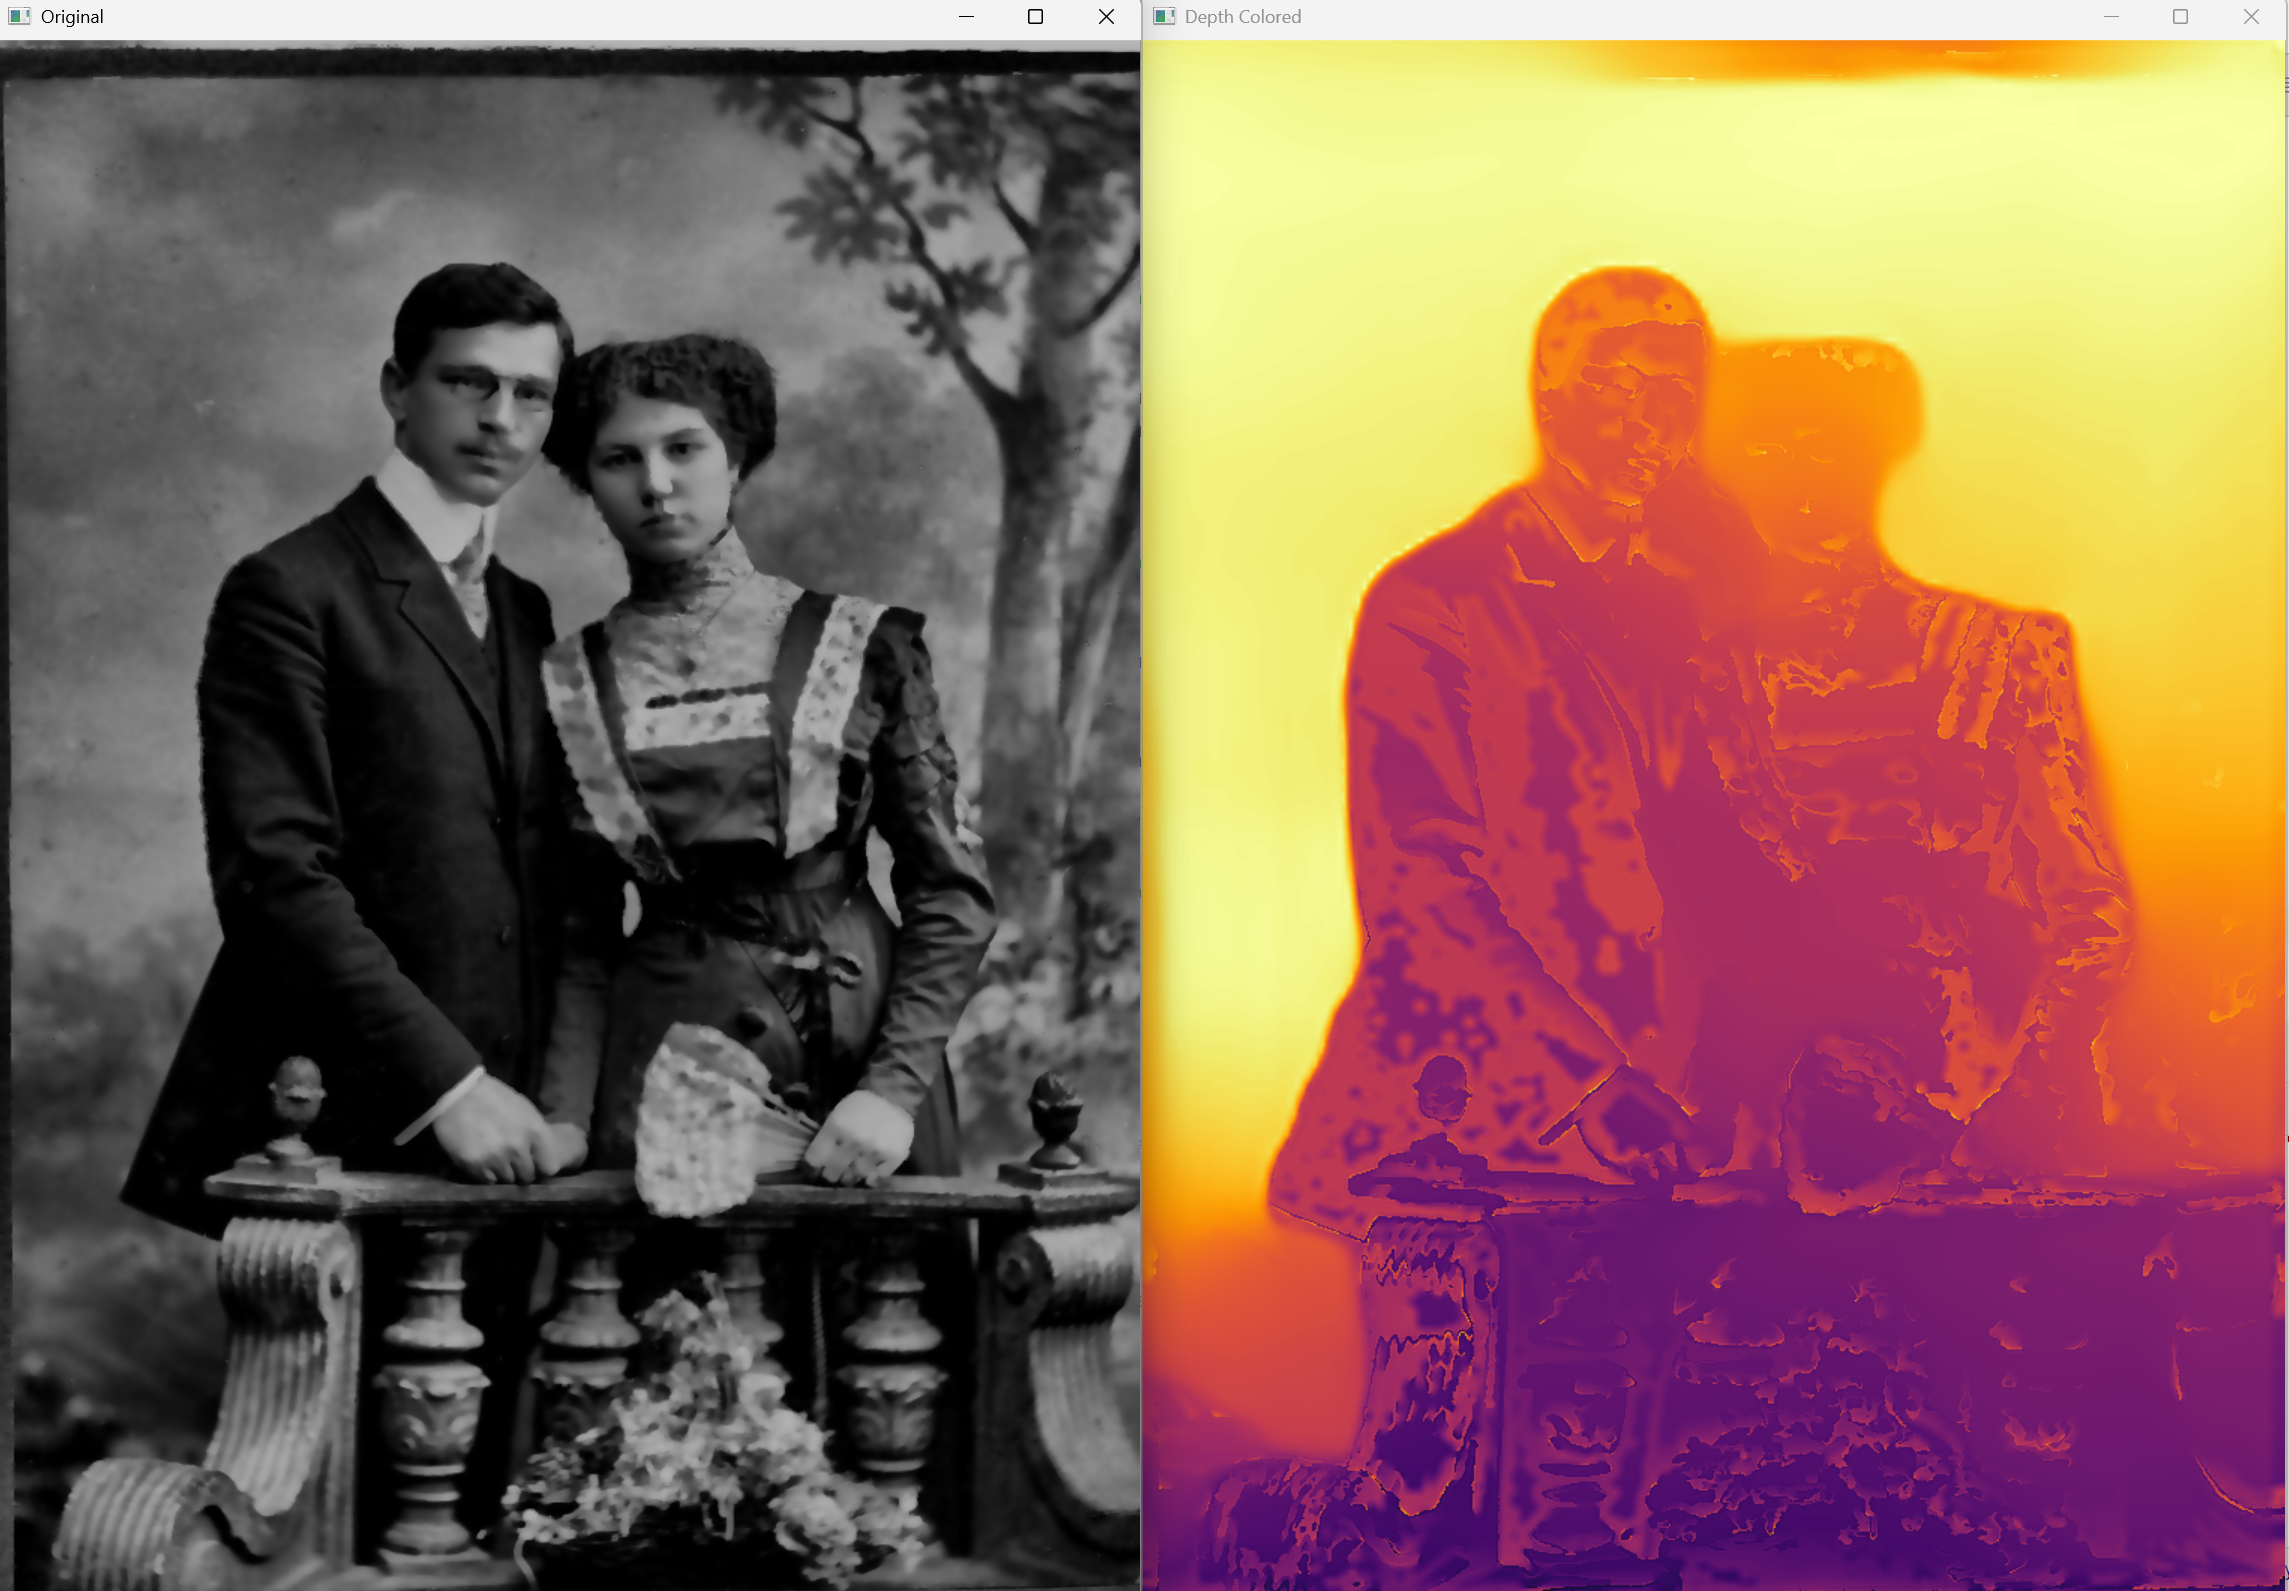
\includegraphics[width=0.9\textwidth]{img/example}
    \caption{Пример визуализации карты глубины: слева -- входное изображение, справа -- предсказанная карта глубин}
    \label{fig:depth_vis}
\end{figure}

\section{Тестирование}

Для обеспечения корректности работы разработанного метода восстановления глубины было проведено модульное тестирование
по методологии "черного ящика" с разделением тестов на классы эквивалентности.

Процесс верификации включает следующие последовательные этапы:
\begin{itemize}
    \item подготовка тестовых изображений, соответствующих каждому классу эквивалентности;
    \item подача на вход метода восстановления глубины пути к тестируемому изображению;
    \item обработка изображения методом восстановления глубины;
    \item визуализация полученной карты глубин в цветовой схеме 'plasma';
    \item сравнение результата с ожидаемым выводом и формирование заключения о корректности.
\end{itemize}

При работе с негативными сценариями дополнительно оценивается корректность обработки исключений,
наличие сообщений об ошибках и соблюдение принципа отказоустойчивости программной системы.
Это гарантирует, что разработанный метод не только правильно функционирует при корректных входных данных,
но и адекватно реагирует на нестандартные ситуации.

В таблице~\ref{tab:test_classes} представлены классы эквивалентности, выделенные для тестирования разработанного метода восстановления глубины из монокулярных изображений.

\begin{table}[H]
    \centering
    \caption{Классы эквивалентности для тестирования}
    \label{tab:test_classes}
    \begin{tabular}{|p{1.5cm}|p{6.5cm}|p{6.5cm}|}
        \hline
        \textbf{Класс} & \textbf{Общее описание} & \textbf{Примеры входных \newline данных} \\
        \hline
        \multicolumn{3}{|l|}{\textbf{Позитивные тесты}} \\
        \hline
        А1 & Обработка черно-белых \newline изображений & Пути к существующим черно-белым изображениям в \newline допустимых форматах (PNG, JPEG) \\
        \hline
        А2 & Обработка изображений в \newline сепии & Пути к существующим \newline изображениям в сепии в \newline допустимых форматах (PNG, JPEG, BMP) \\
        \hline
        А3 & Обработка цветных \newline изображений & Пути к существующим \newline цветным изображениям в \newline допустимых форматах (PNG, JPEG, TIFF) \\
        \hline
        \multicolumn{3}{|l|}{\textbf{Негативные тесты}} \\
        \hline
        Б1 & Обработка отсутствующих файлов & Несуществующие пути к \newline файлам ('/nonexistent.jpg') \\
        \hline
        Б2 & Обработка неподдерживаемых форматов & Пути к файлам с расширениями не из списка допустимых (.txt, .doc) \\
        \hline
        Б3 & Обработка поврежденных изображений & Поврежденные файлы \newline изображений с некорректными данными \\
        \hline
    \end{tabular}
\end{table}

Результаты проведенного тестирования представлены в таблице~\ref{tab:testing_results}.

\begin{table}[H]
    \centering
    \caption{Результаты тестирования метода восстановления глубины}
    \label{tab:testing_results}
    \begin{tabular}{|p{2cm}|p{3.5cm}|p{3.5cm}|p{3.5cm}|p{1.7cm}|}
        \hline
        \textbf{Класс эквив.} & \textbf{Описание входных данных} & \textbf{Ожидаемый результат} & \textbf{Полученный результат} & \textbf{Статус} \\
        \hline
        А1 & Черно-белое изображение в формате JPEG & Успешная загрузка и генерация карты глубины & Карта глубины сгенерирована, сохранена и визуализирована & Пройден \\
        \hline
        А1 & Черно-белое изображение в формате PNG & Успешная загрузка и генерация карты глубины & Карта глубины сгенерирована, сохранена и визуализирована & Пройден \\
        \hline
        А2 & Изображение с эффектом сепии в формате BMP & Успешная загрузка и генерация карты глубины & Карта глубины сгенерирована, сохранена и визуализирована & Пройден \\
        \hline
        А3 & Цветное изображение размером 4K (3840×2160) & Успешная обработка с автоматическим масштабированием & Изображение масштабировано и обработано корректно & Пройден \\
        \hline
        Б1 & Путь к несуществующему файлу ('/nonexistent.jpg') & Сообщение об ошибке с указанием на отсутствие файла & "Ошибка: файл '/nonexistent.jpg' не существует" & Пройден \\
        \hline
        Б2 & Путь к файлу с расширением .txt & Сообщение о неподдерживаемом формате файла & "Ошибка: формат '.txt' не поддерживается" & Пройден \\
        \hline
        Б3 & Поврежденный JPEG-файл & Сообщение о невозможности декодирования изображения & "Ошибка при декодировании изображения" & Пройден \\
        \hline
    \end{tabular}
\end{table}

Проведенное тестирование показало, что разработанный метод корректно обрабатывает изображения различных поддерживаемых форматов,
а также адекватно реагирует на некорректные входные данные, предоставляя пользователю информативные сообщения об ошибках.

\section{Вывод}
В технологическом разделе выполнена полная программная реализация гибридного метода восстановления глубины из монокулярных изображений.

Для решения поставленной задачи был выбран язык Python с экосистемой специализированных библиотек (OpenCV, PyTorch, NumPy и др.),
что обеспечило эффективную работу с изображениями, применение моделей машинного обучения и визуализацию трехмерных данных.

Разработанный алгоритм успешно прошел тестирование на различных типах изображений (цветных, черно-белых, с эффектом сепии)
и продемонстрировал корректную обработку исключительных ситуаций, что подтверждает работоспособность созданного решения.


    \chapter{Исследовательский раздел}

% TODO красиво оформить список источников
% TODO Отладить код так, чтобы было что показать на защите
% TODO Презентацию сделать
%% TODO Добавить датасет с людьми в часть с кодом

Цель данного исследования --- объективная оценка качества реконструкции глубины посредством разработанного гибридного метода по сравнению с современными подходами, с особым вниманием к устойчивости методов при работе с деградировавшими изображениями. Исследование направлено на определение сильных и слабых сторон разработанного метода, а также его применимости к архивным фотографиям с различными характеристиками.

Основные задачи исследования:
\begin{itemize}
    \item проанализировать влияние различных типов деградации изображений на качество реконструкции;
    \item сравнить точность восстановления глубины разработанного метода с современными подходами на эталонных наборах данных;
    \item определить наиболее подходящие области применения каждого метода.
\end{itemize}

\section{Описание входных данных}

Ввиду отсутствия эталонных данных о глубине для архивных фотографий,
разработан методологический подход с использованием современных датасетов с верифицированными картами глубины и алгоритмов искусственного старения,
позволяющий количественно оценивать результаты реконструкции в контролируемых условиях.

Для проведения исследования были выбраны следующие датасеты, обеспечивающих разнообразие тестовых сцен:

\begin{enumerate}
    \item \textbf{NYU Depth v2} --- 1449 изображений внутренних помещений с глубиной, полученной с помощью сенсора Kinect~\cite{silberman2012indoor}.
    \item \textbf{4D Light Field Benchmark} --- 24 синтетические сцены с глубиной, полученной с помощью рендеринга 3D-моделей~\cite{honauer2017dataset}.
    \item \textbf{BIWI Kinect Head Pose} --- набор из более 15000 изображений 20 человек, полученных с помощью сенсора Kinect~\cite{fanelli_IJCV}.
\end{enumerate}

Из каждого датасета было случайным образом отобрано по 20 изображений,
обеспечивая статистическую значимость результатов при сохранении выполнимости тестирования в разумные сроки.

Для имитации состаривания изображений был разработан программный модуль, реализующий следующие эффекты с параметрически задаваемой интенсивностью (от 0 до 1):

\begin{itemize}
     \item \textbf{сепия} --- преобразование RGB в тонированное монохромное изображение,
     \item \textbf{виньетирование} --- затемнение краев изображения,
     \item \textbf{шум и зернистость} --- добавление шума, имитирующего фотопленку,
     \item \textbf{выцветание} --- снижение контраста и насыщенности,
     \item \textbf{случайные пятна и царапины} --- добавление локальных дефектов.
\end{itemize}

\section{Метрики оценки качества}

% TODO надо ли описание элементоов формулы оформлять в виде списка или и так сойдет?

Для объективной оценки качества восстановления глубины используются метрики, которые позволяют количественно оценить,
насколько точно модель предсказывает карту глубины, сравнивая предсказанные значения с истинными.

Для корректного сравнения методов, формирующих результаты в разных масштабах, в работе используется предварительная нормализация карт глубин, которая выполняется по формуле:
\begin{equation}
    d_{\text{norm}} = \frac{d - d_{\text{min}}}{d_{\text{max}} - d_{\text{min}}},
\end{equation}
$d_{\text{norm}}$ --- нормализованное значение глубины, 
$d$ --- исходное значение глубины, 
$d_{\text{min}}$ --- минимальное значение глубины в карте глубин, 
$d_{\text{max}}$ --- максимальное значение глубины в карте глубин. 

Для определения среднего отклонения результата используется метрика $RMSE$ --- среднеквадратичное отклонение результата
(от англ. Root Mean Square Error), которая позволяет оценить,
насколько предсказанные значения глубины отличны от истинных значений в среднем по всем пикселям изображения~\cite{zhang2025review, istomin2024, shestopalov2024}.
$RMSE$ вычисляется согласно формуле:

\begin{equation}
    \text{RMSE} = \sqrt{\frac{1}{n} \sum_{i=1}^{n} (d_{i}^{\text{pred}} - d_{i}^{\text{gt}})^2},
\end{equation}
 где $n$ -- общее количество пикселей изображения,
$d_{i}^{\text{pred}}$ -- предсказанное значение глубины для $i$-го пикселя,
$d_{i}^{\text{gt}}$ -- истинное (эталонное) значение глубины для $i$-го пикселя.

С учетом нормализации, минимальное значение RMSE --- 0, максимальное --- 1.
Чем ближе значение метрики к 0, тем точнее предсказание.

С целью определения количества предсказанных значений глубины, которые находятся в пределах допустимого отклонения используется
пороговая относительная точность ($\delta_{\lambda}$)~\cite{zhang2025review, istomin2024, shestopalov2024}.
Эта метрика измеряет долю пикселей, для которых предсказанные и истинные значения глубины удовлетворяют следующему условию:

\begin{equation} 
    \max\left(\frac{d_{i}^{\text{pred}}}{d_{i}^{\text{gt}}}, \frac{d_{i}^{\text{gt}}}{d_{i}^{\text{pred}}}\right) = \delta < t_{\lambda} 
\end{equation}

где $d_{i}^{\text{gt}}$ --- истинное значение глубины для $i$-го пикселя,
$d_{i}^{\text{pred}}$ --- предсказанное значение глубины для $i$-го пикселя,
$\delta$ --- значение, показывающее отклонение предсказанного значения от истинного,
$t_{\lambda}$ --- пороговое значение, при котором отклонение считается допустимым.

В работе используются пороги $\lambda=1,2,3$, что соответствует отклонению в 25\%, 56.25\% и 95.3\% соответственно.

С учетом нормализации значения метрики $\delta_{\lambda}$ лежат в диапазоне от 0 до 1.
Чем ближе значение метрики к 1, тем большая доля пикселей имеет точное предсказание глубины в пределах соответствующего порога.

\section{Исследование устойчивости метода к деградации изображений}

Исследуется эффективность гибридного метода в зависимости от интенсивности различных эффектов старения,
применённых к тестовым изображениям изолированно.

Для каждого эффекта (сепия, виньетирование, шум, выцветание, пятна) применялись различные уровни интенсивности от 0.0 до 1.0 с шагом 0.2.

Гипотеза заключается в том, что различные эффекты старения будут по-разному влиять на точность реконструкции глубины:
эффекты, изменяющие только цветовую гамму изображения (сепия, выцветание), окажут меньшее влияние на точность,
чем эффекты, искажающие структурную информацию изображения (шум, пятна, виньетирование).

На рисунке~\ref{fig:effects-rmse} представлены графики зависимости среднеквадратичной ошибки от интенсивности применения различных эффектов старения к тестовым изображениям.

\begin{figure}
\centering
    \begin{tikzpicture}
        \begin{axis}[
            width=0.9\textwidth,
            height=6cm,
            xlabel={Интенсивность эффекта},
            ylabel={Среднеквадратичная ошибка (RMSE)},
            xmin=-0.05, xmax=1.05,
            ymin=0.21, ymax=0.33,
            xtick={0,0.2,0.4,0.6,0.8,1.0},
            grid=both,
            grid style={line width=.1pt, draw=gray!10},
            major grid style={line width=.2pt,draw=gray!50},
            every axis plot/.append style={smooth},
            legend pos=north west,
            legend style={font=\small},
            legend columns=2]

            % Сепия
            \addplot[black, solid, smooth] coordinates {
                (0.0, 0.22673959517265008)
                (0.2, 0.2224120524354949)
                (0.4, 0.22380517749733062)
                (0.6, 0.22040347321392373)
                (0.8, 0.22158114785240235)
                (1.0, 0.22479423061609816)
            };

            % Виньетирование
            \addplot[black, dashed, smooth] coordinates {
                (0.0, 0.22673959517265008)
                (0.2, 0.256956901702622)
                (0.4, 0.2672339682435893)
                (0.6, 0.27263466877343556)
                (0.8, 0.2877002885964059)
                (1.0, 0.2835513838997222)
            };

            % Шум
            \addplot[black, dotted, smooth, line width=1.25pt] coordinates {
                (0.0, 0.22673959517265008)
                (0.2, 0.22550388966890234)
                (0.4, 0.2474848386682945)
                (0.6, 0.312124558133447)
                (0.8, 0.32290318666871687)
                (1.0, 0.2973997438450658)
            };

            % Выцветание
            \addplot[black, dashdotted, smooth] coordinates {
                (0.0, 0.22673959517265008)
                (0.2, 0.22192686388303162)
                (0.4, 0.21995908234551922)
                (0.6, 0.22126814934419525)
                (0.8, 0.23044226142223376)
                (1.0, 0.22065211351964661)
            };

            % Пятна
            \addplot[black, loosely dashed, smooth] coordinates {
                (0.0, 0.22673959517265008)
                (0.2, 0.24074089383533015)
                (0.4, 0.23506201341607524)
                (0.6, 0.2461171888472462)
                (0.8, 0.24989895793232644)
                (1.0, 0.2392362046372416)
            };

            \legend{Сепия, Виньетирование, Шум, Выцветание, Пятна}
        \end{axis}
    \end{tikzpicture}
    \caption{Влияние эффектов старения на среднеквадратичную ошибку (RMSE)}
    \label{fig:effects-rmse}
\end{figure}

Анализ полученных данных подтверждает выдвинутую гипотезу о том, что эффекты, изменяющие только цветовую гамму изображения (сепия, выцветание),
оказывают меньшее влияние на точность реконструкции, чем эффекты, искажающие структурную информацию (шум, виньетирование, пятна).

\begin{enumerate}
    \item \textbf{Сепия и выцветание} оказывают минимальное влияние на точность метода:
    при максимальной интенсивности эффектов для сепии отклонение RMSE составляет 0.0006 (0.26\%), для выцветания — 0.004 (1.6\%).
    Это объясняется тем, что преобразования цветовой гаммы не изменяют структурную информацию изображения, а алгоритмы восстановления глубины опираются преимущественно на структурные, а не цветовые характеристики.

    \item \textbf{Виньетирование} демонстрирует значительно более выраженное влияние:
    при интенсивности 0.8 наблюдается максимальное увеличение RMSE на 0.061 (26.8\%).
    Затемнение по краям изображения существенно влияет на восприятие глубины, особенно в периферийных областях, что подтверждает гипотезу о важности равномерного освещения для структурного анализа изображения.

    \item \textbf{Шум} показывает наиболее сильное влияние на точность реконструкции:
    при интенсивности 0.8 RMSE возрастает на 0.096 (42.4\%).
    Шум разрушает текстуры и размывает границы объектов, что критически затрудняет анализ формы из затенения и работу нейросетевых алгоритмов.

    \item \textbf{Пятна и царапины} демонстрируют умеренное, но устойчивое влияние на точность:
    максимальное увеличение RMSE на 0.023 (10.2\%) наблюдается при интенсивности 0.8.
    Локальные искажения структуры изображения влияют на алгоритм менее критично, чем равномерный шум, но более существенно, чем изменения цветовой гаммы.
\end{enumerate}

Результаты позволяют определить наиболее эффективные области применения разработанного метода:
реконструкция трёхмерной информации из фотографий с преимущественно цветовой деградацией (сепия, выцветание) и умеренными локальными дефектами.
В то же время для изображений с сильным шумом или виньетированием необходима более тщательная предварительная обработка.

\section{Сравнительный анализ методов}

В данном исследовании сравнивалась три метода восстановления глубины из монокулярных изображений:
\begin{itemize}
    \item \textbf{восстановление глубины по закраске изображения (SFS)} --- метод, основанный на анализе формы из затенения (Shape From Shading), использующий информацию о характере освещения для восстановления формы объектов;
    \item \textbf{MiDaS} --- метод восстановления глубины на основе глубоких нейронных сетей, обученный на разнородных данных для повышения обобщающей способности;
    \item \textbf{гибридный метод} --- разработанный в рамках исследования подход, адаптивно интегрирующий нейросетевой метод MiDaS и классический метод Shape From Shading.
\end{itemize}

С целью комплексного исследования влияния деградации изображений на качество восстановления глубины
применялась методика контролируемого искусственного старения.
Эффекты деградации моделировались с различными интенсивностями: для виньетирования и пятен — в диапазоне от 0 до 0.6, а для сепии и выцветания — от 0 до 1.0, что основано на результатах предыдущего исследования.

Гипотеза заключается в том, что гибридный метод будет объединять преимущества обоих подходов:
стабильность MiDaS при работе с деградированными изображениями и высокую детализацию SFS на качественных изображениях. 
Ожидается, что при увеличении степени деградации изображений гибридный метод будет демонстрировать большую устойчивость, 
чем чистый SFS, сохраняя при этом лучшую точность восстановления геометрических деталей по сравнению с чистым MiDaS.

В таблице~\ref{tab:comparison-by-degradation} представлены результаты сравнения трех методов по метрикам RMSE и $\delta_{\lambda}$ при различных уровнях деградации изображений.

\begin{table}[H]
\centering
\caption{Сравнение методов восстановления глубины при различных уровнях деградации изображений}
\label{tab:comparison-by-degradation}
\begin{tabular}{|l|c|c|c|c|c|}
\hline
\textbf{Метод} & \textbf{Уровень} & \textbf{RMSE} & \textbf{$\delta_1$} & \textbf{$\delta_2$} & \textbf{$\delta_3$} \\
\hline
\multirow{Гибридный} & 0 & 0.2854 & 0.6376 & 0.8739 & 0.9760 \\
 & 1 & 0.2954 & 0.6380 & 0.8666 & 0.9677 \\
 & 2 & 0.2931 & 0.6849 & 0.8863 & 0.9667 \\
 & 3 & 0.2918 & 0.6415 & 0.8638 & 0.9565 \\
\hline
\multirow{MiDaS} & 0 & 0.2914 & 0.6425 & 0.8597 & 0.9542 \\
 & 1 & 0.2947 & 0.6399 & 0.8607 & 0.9542 \\
 & 2 & 0.2983 & 0.6715 & 0.8735 & 0.9522 \\
 & 3 & 0.2979 & 0.6438 & 0.8646 & 0.9427 \\
\hline
\multirow{SFS} & 0 & 0.2867 & 0.6768 & 0.8866 & 0.9790 \\
 & 1 & 0.3832 & 0.3664 & 0.5749 & 0.7588 \\
 & 2 & 0.3959 & 0.3749 & 0.6144 & 0.7667 \\
 & 3 & 0.4170 & 0.4133 & 0.6090 & 0.7622 \\
\hline
\end{tabular}
\end{table}

На рисунках~\ref{fig:comparison-rmse}, ~\ref{fig:comparison-by-degradation} представлены графики, визуализирующие результаты исследования.

\begin{figure}[H]
\centering
    \begin{tikzpicture}
        \begin{axis}[
            width=\textwidth,
            height=6cm,
            xlabel={Уровень деградации},
            ylabel={Среднеквадратичная ошибка (RMSE)},
            xmin=-0.1, xmax=3.1,
            ymin=0.25, ymax=0.6,
            xtick={0,1,2,3},
            ytick={0.3,0.35,0.4,0.45,0.5,0.55,0.6},
            grid=both,
            grid style={line width=.1pt, draw=gray!10},
            major grid style={line width=.2pt,draw=gray!50},
            legend pos=north east,
            legend style={font=\small}]

            % Гибридный метод
            \addplot[black, mark=*, smooth] coordinates {
                (0, 0.28541211159480284)
                (1, 0.295440172140253)
                (2, 0.2931316731338902)
                (3, 0.2918331874608755)
            };

            % MiDaS
            \addplot[black, dashed, mark=square*, smooth] coordinates {
                (0, 0.29138717467995495)
                (1, 0.2947147948982483)
                (2, 0.29826661689549494)
                (3, 0.2979285750148052)
            };

            % SFS (Segmentation)
            \addplot[black, dotted, mark=triangle*, smooth] coordinates {
                (0, 0.2867484161955488)
                (1, 0.3832440906946321)
                (2, 0.39591868578935213)
                (3, 0.4169904701291959)
            };

            \legend{Гибридный метод, MiDaS, SFS}
        \end{axis}
    \end{tikzpicture}
    \caption{Сравнение методов по метрике RMSE при различных уровнях деградации}
    \label{fig:comparison-rmse}
\end{figure}

\begin{figure}[H]
\centering
    \begin{tikzpicture}
        \begin{axis}[
            width=\textwidth,
            height=8cm,
            xlabel={Уровень деградации},
            ylabel={Значение метрик $\delta_{\lambda}$},
            xmin=-0.5, xmax=3.5,
            ymin=0.35, ymax=1,
            xtick={0,1,2,3},
            ytick={0.4,0.5,0.6,0.7,0.8,0.9, 1},
            grid=both,
            grid style={line width=.1pt, draw=gray!10},
            major grid style={line width=.2pt,draw=gray!50},
            legend style={font=\small,at={(0.5,-0.25)},anchor=north,legend columns=3},
            legend cell align={left}]

            % Гибридный метод - Delta1
            \addplot[black, mark=*, smooth] coordinates {
                (0, 0.6376040039062501)
                (1, 0.6380177408854165)
                (2, 0.6849495442708332)
                (3, 0.6414757486979165)
            };

            % MiDaS - Delta1
            \addplot[black, dashed, mark=*, smooth] coordinates {
                (0, 0.6425073242187499)
                (1, 0.6399417317708334)
                (2, 0.6715174153645833)
                (3, 0.6438002929687499)
            };

            % SFS - Delta1
            \addplot[black, dotted, mark=*, smooth] coordinates {
                (0, 0.6767942708333333)
                (1, 0.36636621093749996)
                (2, 0.3749396158854167)
                (3, 0.41326790364583335)
            };

            % Гибридный метод - Delta2
            \addplot[black, mark=square*, smooth] coordinates {
                (0, 0.8739314778645833)
                (1, 0.8665922851562499)
                (2, 0.8863361002604167)
                (3, 0.8638222656250001)
            };

            % MiDaS - Delta2
            \addplot[black, dashed, mark=square*, smooth] coordinates {
                (0, 0.8597228190104166)
                (1, 0.8607184244791665)
                (2, 0.8735188802083333)
                (3, 0.8645610351562502)
            };

            % SFS - Delta2
            \addplot[black, dotted, mark=square*, smooth] coordinates {
                (0, 0.8865755208333334)
                (1, 0.57492626953125)
                (2, 0.6144095052083333)
                (3, 0.6090374348958332)
            };

            % Гибридный метод - Delta3
            \addplot[black, mark=triangle*, smooth] coordinates {
                (0, 0.9759777018229167)
                (1, 0.9676751302083334)
                (2, 0.9666614583333334)
                (3, 0.9564737955729166)
            };

            % MiDaS - Delta3
            \addplot[black, dashed, mark=triangle*, smooth] coordinates {
                (0, 0.9542218424479169)
                (1, 0.9541813151041666)
                (2, 0.9522010091145832)
                (3, 0.9427171223958334)
            };

            % SFS - Delta3
            \addplot[black, dotted, mark=triangle*, smooth] coordinates {
                (0, 0.9790131835937501)
                (1, 0.7588245442708333)
                (2, 0.76665478515625)
                (3, 0.7621984049479166)
            };

            \legend{$\delta_1$ Гибридный, $\delta_1$ MiDaS, $\delta_1$ SFS,
                    $\delta_2$ Гибридный, $\delta_2$ MiDaS, $\delta_2$ SFS,
                    $\delta_3$ Гибридный, $\delta_3$ MiDaS, $\delta_3$ SFS}
        \end{axis}
    \end{tikzpicture}
    \caption{Сравнение методов по метрикам $\delta_{\lambda}$ при различных уровнях деградации}
    \label{fig:comparison-by-degradation}
\end{figure}

На качественных изображениях (уровень деградации 0) все три метода показывают сопоставимые результаты по метрике RMSE: 
гибридный метод (0.2854), SFS (0.2867) и MiDaS (0.2914).
При этом SFS демонстрирует наилучшие показатели по метрикам $\delta_1$, $\delta_2$ и $\delta_3$.

При увеличении уровня деградации (уровни 1-3) наблюдается следующая динамика:
\begin{itemize}
    \item метод SFS критически теряет в точности: RMSE возрастает на 45.4\%, а метрики $\delta_1$, $\delta_2$ и $\delta_3$ падают на 39-41\%;
    \item MiDaS демонстрирует стабильные показатели: RMSE практически не изменяется (0.2947-0.2983), как и метрики $\delta_\lambda$;
    \item гибридный метод сохраняет устойчивость на уровне MiDaS, но с лучшими абсолютными показателями:
RMSE в диапазоне 0.2918-0.2954 и метрики $\delta_2$ и $\delta_3$ в пределах 0.8638-0.8863 и 0.9565-0.9677 соответственно.
\end{itemize}

Результаты сравнительного анализа трех методов восстановления глубины подтверждают выдвинутую гипотезу: по сравнению с базовыми методами
гибридный демонстрирует незначительное повышение точности (около 1-2\%), которое стабильно наблюдается на всех уровнях деградации изображений.


Полученные результаты позволяют определить оптимальные области применения каждого из методов.
\begin{itemize} \item \textbf{SFS} наиболее эффективен при работе с качественными изображениями без деградации, где обеспечивает высокую детализацию поверхностей. Рекомендуется для применения в контролируемых условиях, например, в промышленных системах контроля качества или при работе с современными цифровыми изображениями высокого разрешения;
\item \textbf{MiDaS} демонстрирует универсальность и устойчивость к различным типам искажений, что делает его подходящим для обработки разнородных коллекций изображений. Оптимален для задач, где важна стабильность результатов, но высокая детализация не является критичной;
\item \textbf{Гибридный метод} обеспечивает оптимальный баланс между устойчивостью к деградации и детализацией при восстановлении трёхмерной информации из архивных фотографий. Метод повышает точность реконструкции без необходимости переобучения нейросетевых моделей, что существенно снижает вычислительные затраты.
\end{itemize}

\section*{Вывод}

% TODO переписать

В исследовательском разделе проведено исследование с использованием стандартных датасетов,
алгоритмов искусственного старения изображений и объективных метрик оценки
для количественной оценки эффективности разработанного гибридного метода восстановления глубины.

Проведено исследование устойчивости гибридного метода к различным эффектам старения изображений,
которое подтвердило гипотезу о дифференцированном влиянии различных типов деградации на точность реконструкции глубины:
    \begin{itemize}
        \item эффекты, изменяющие структурную информацию (шум и виньетирование), оказывают наиболее сильное негативное влияние (26.8-42.4\% увеличения RMSE);
        \item эффекты, затрагивающие только цветовую гамму (сепия и выцветание), влияют минимально (0.26-1.6\% увеличения RMSE);
        \item локальные искажения (пятна и царапины) оказывают умеренное влияние (около 10.2\% увеличения RMSE).
    \end{itemize}

Результаты позволяют определить наиболее эффективные области применения разработанного метода:
реконструкция трёхмерной информации из фотографий с преимущественно цветовой деградацией (сепия, выцветание) и умеренными локальными дефектами.
В то же время для изображений с сильным шумом или виньетированием необходима более тщательная предварительная обработка.

Выполнен сравнительный анализ разработанного гибридного метода с базовыми подходами (MiDaS и SFS) при различных уровнях деградации изображений:
    \begin{itemize}
        \item на качественных изображениях все три метода демонстрируют сопоставимые результаты по метрике RMSE;
        \item при увеличении уровня деградации метод SFS критически теряет в точности (RMSE возрастает на 45.4\%);
        \item MiDaS сохраняет стабильность на всех уровнях деградации;
        \item гибридный метод демонстрирует устойчивость на уровне MiDaS с улучшенными на 1-2\% абсолютными показателями точности.
    \end{itemize}

Полученные результаты позволяют определить оптимальные области применения каждого из методов.
\begin{itemize} \item \textbf{SFS} наиболее эффективен при работе с качественными изображениями без деградации, где обеспечивает высокую детализацию поверхностей. Рекомендуется для применения в контролируемых условиях, например, в промышленных системах контроля качества или при работе с современными цифровыми изображениями высокого разрешения;
\item \textbf{MiDaS} демонстрирует универсальность и устойчивость к различным типам искажений, что делает его подходящим для обработки разнородных коллекций изображений. Оптимален для задач, где важна стабильность результатов, но высокая детализация не является критичной;
\item \textbf{Гибридный метод} обеспечивает оптимальный баланс между устойчивостью к деградации и детализацией при восстановлении трёхмерной информации из архивных фотографий. Метод повышает точность реконструкции без необходимости переобучения нейросетевых моделей, что существенно снижает вычислительные затраты.
\end{itemize}

Результаты исследования подтверждают эффективность разработанного гибридного метода,
который успешно сочетает в себе устойчивость нейросетевого подхода к деградации изображений с детализирующими возможностями метода Shape from Shading.

Полученные данные позволяют определить оптимальные области применения метода:
восстановление трёхмерной информации из архивных фотографий для задач цифровой реставрации и трёхмерной реконструкции исторических объектов,
когда доступны только архивные фотоматериалы различного качества, но с минимальным уровнем шумовых искажений.
Метод позволяет получить более точные и детализированные карты глубины по сравнению с существующими подходами.



    \chapter*{ЗАКЛЮЧЕНИЕ}
\addcontentsline{toc}{chapter}{ЗАКЛЮЧЕНИЕ}



В аналитической части работы был проведен анализ существующих методов конвертации двумерных изображений в трехмерные представления.
Методы были классифицированы по ключевым критериям: способу получения данных, типу исходных изображений, необходимости в дополнительной информации, результатам реконструкции, масштабу сцены и уровню автоматизации.

В ходе исследования были изучены различные подходы к восстановлению 3D-информации,
включая методы структурированного освещения, стерео сопоставления, DFD, Shape from Shading, Comfortable Depth Generation и нейросетевые методы, такие как MiDaS.

Проведенный анализ привел к выводу, что оптимальным решением для восстановления глубины из архивных фотографий является гибридный метод,
объединяющий преимущества нейросетевого подхода (MiDaS) и классического метода Shape from Shading.
Такое решение позволит обеспечить как общую точность восстановления геометрии сцены, так и детализацию отдельных элементов, сохраняя при этом устойчивость к дефектам, характерным для исторических изображений.

Представленная формальная модель задачи и декомпозиция метода на функциональные блоки предобработки, гибридного восстановления и постобработки формируют теоретическую основу для разработки практического решения в следующих разделах работы.



В конструкторском разделе была представлена детальная структура разработанного гибридного метода восстановления трехмерной информации из архивных фотографий.
Разработка включает семь основных алгоритмических блоков, последовательное выполнение которых обеспечивает преобразование входного изображения в детализированную карту глубины.

Представленные схемы алгоритмов являются основой для последующей программной реализации метода, которая будет рассмотрена в технологическом разделе работы.

В технологическом разделе выполнена полная программная реализация гибридного метода восстановления глубины из монокулярных изображений.

Для решения поставленной задачи был выбран язык Python с экосистемой специализированных библиотек (OpenCV, PyTorch, NumPy и др.),
что обеспечило эффективную работу с изображениями, применение моделей машинного обучения и визуализацию трехмерных данных.

Разработанный алгоритм успешно прошел тестирование на различных типах изображений (цветных, черно-белых, с эффектом сепии)
и продемонстрировал корректную обработку исключительных ситуаций, что подтверждает работоспособность созданного решения.



В исследовательском разделе проведено исследование с использованием стандартных датасетов,
алгоритмов искусственного старения изображений и объективных метрик оценки
для количественной оценки эффективности разработанного гибридного метода восстановления глубины.

Проведено исследование устойчивости гибридного метода к различным эффектам старения изображений,
которое подтвердило гипотезу о дифференцированном влиянии различных типов деградации на точность реконструкции глубины:
    \begin{itemize}
        \item эффекты, изменяющие структурную информацию (шум и виньетирование), оказывают наиболее сильное негативное влияние (26.8-42.4\% увеличения RMSE);
        \item эффекты, затрагивающие только цветовую гамму (сепия и выцветание), влияют минимально (0.26-1.6\% увеличения RMSE);
        \item локальные искажения (пятна и царапины) оказывают умеренное влияние (около 10.2\% увеличения RMSE).
    \end{itemize}

Выполнен сравнительный анализ разработанного гибридного метода с базовыми подходами (MiDaS и SFS) при различных уровнях деградации изображений:
    \begin{itemize}
        \item на качественных изображениях все три метода демонстрируют сопоставимые результаты по метрике RMSE;
        \item при увеличении уровня деградации метод SFS критически теряет в точности (RMSE возрастает на 45.4\%);
        \item MiDaS сохраняет стабильность на всех уровнях деградации;
        \item гибридный метод демонстрирует устойчивость на уровне MiDaS с улучшенными на 1-2\% абсолютными показателями точности.
    \end{itemize}

Результаты исследования подтверждают эффективность разработанного гибридного метода,
который успешно сочетает в себе устойчивость нейросетевого подхода к деградации изображений с детализирующими возможностями метода Shape from Shading.
Полученные данные позволяют определить оптимальные области применения метода:
восстановление трёхмерной информации из архивных фотографий для задач цифровой реставрации и трёхмерной реконструкции исторических объектов,
когда доступны только архивные фотоматериалы различного качества.
Метод позволяет получить более точные и детализированные карты глубины по сравнению с существующими подходами при работе с деградированными изображениями.


экономическую эффективность или значимость работы;
 прогнозы и предположения о возможных направлениях развития объекта
исследования.


    %\renewcommand \bibname{СПИСОК ИСПОЛЬЗОВАННЫХ ИСТОЧНИКОВ} % переименовать страницу списка литературы
%%\bibliographystyle{utf8gost705u}  % стилевой файл для оформления по ГОСТу
%

\makebibliography


    \begin{appendices}
    \chapter{}
    Презентация к научно--исследовательской работе содержит 11 слайдов.
\end{appendices}



\end{document}